\documentclass[3pt,a5paper,openright,twoside]{book}
% \documentclass[12pt,a5paper,openright,twoside]{book}

\oddsidemargin=10pt \evensidemargin=-10pt

\usepackage{multicol}
\usepackage{layout}
\usepackage[usenames, dvipsnames]{color}



% !Mode:: "TeX:UTF-8"
%  Authors: 张井   Jing Zhang: prayever@gmail.com     天津大学2010级管理与经济学部信息管理与信息系统专业硕士生
%           余蓝涛 Lantao Yu: lantaoyu1991@gmail.com  天津大学2008级精密仪器与光电子工程学院测控技术与仪器专业本科生

%%%%%%%%%% Package %%%%%%%%%%%%
% \usepackage[utf8]{inputenc}
\usepackage{tabularx}
\usepackage{float}

\usepackage{caption}
\usepackage{subcaption}
\usepackage{algpseudocode}
\usepackage{algorithm}
\usepackage{mathtools}
\usepackage{hyperref}
\usepackage{fancyhdr}
\usepackage{indentfirst}
\usepackage{graphicx}
\usepackage{newlfont}
\usepackage{amssymb}
\usepackage{amsmath}
\usepackage{latexsym}
\usepackage{amsthm}
\usepackage[UTF8]{ctex}                     % 支持中文显示
\usepackage{CJKutf8}                        % 用在UTF8编码环境下,它可以自动调用CJK,同时针对UTF8编码作了设置。
\usepackage{pdfpages}


% \usepackage{lipsum}

% without chapter
% \usepackage{titlesec}
% \titleformat{\chapter}[display]
%   {\normalfont\bfseries}{章节}{0pt}{\Large}

% chapter in Chinese
% \usepackage[english]{babel}
% \addto\captionsenglish{\renewcommand{\chaptername}{章节}}



\hyphenation{sil-la-ba-zio-ne pa-ren-te-si}

\pagestyle{fancy}\addtolength{\headwidth}{20pt}
\renewcommand{\chaptermark}[1]{\markboth{\thechapter.\ #1}{}}
\renewcommand{\sectionmark}[1]{\markright{\thesection \ #1}{}}
\rhead[\fancyplain{}{\bfseries\leftmark}]{\fancyplain{}{\bfseries\thepage}}

\renewcommand{\footrulewidth}{0.4pt}
\cfoot{博洛尼亚留学手册2018版}
% \linespread{1.1}         


% \usepackage{graphicx}                       % 支持插图处理
% \usepackage[a4paper,text={150true mm,224true mm},top=35.5true mm,left=30true mm,head=5true mm,headsep=2.5true mm,foot=8.5true mm]{geometry}
                                            % 支持版面尺寸设置
\usepackage{titlesec}                       % 控制标题的宏包
\usepackage{titletoc}                       % 控制目录的宏包
% \usepackage{fancyhdr}                       % fancyhdr宏包 支持页眉和页脚的相关定义
\usepackage[UTF8]{ctex}                     % 支持中文显示
% \usepackage{color}                          % 支持彩色
% \usepackage{amsmath}                        % AMSLaTeX宏包 用来排出更加漂亮的公式
% \usepackage{amssymb}                        % 数学符号生成命令
% \usepackage[below]{placeins}                %允许上一个section的浮动图形出现在下一个section的开始部分,还提供\FloatBarrier命令,使所有未处理的浮动图形立即被处理
% \usepackage{flafter}                        % 使得所有浮动体不能被放置在其浮动环境之前,以免浮动体在引述它的文本之前出现.
% \usepackage{multirow}                       % 使用Multirow宏包,使得表格可以合并多个row格
% \usepackage{booktabs}                       % 表格,横的粗线;\specialrule{1pt}{0pt}{0pt}
% \usepackage{longtable}                      % 支持跨页的表格。
% \usepackage{tabularx}                       % 自动设置表格的列宽
% \usepackage{subfigure}                      % 支持子图 %centerlast 设置最后一行是否居中
% \usepackage[subfigure]{ccaption}            % 支持子图的中文标题
% \usepackage[sort&compress,numbers]{natbib}  % 支持引用缩写的宏包
% \usepackage{enumitem}                       % 使用enumitem宏包,改变列表项的格式
% \usepackage{calc}                           % 长度可以用+ - * / 进行计算
% \usepackage{txfonts}                        % 字体宏包
% \usepackage{bm}                             % 处理数学公式中的黑斜体的宏包
% \usepackage[amsmath,thmmarks,hyperref]{ntheorem}  % 定理类环境宏包,其中 amsmath 选项用来兼容 AMS LaTeX 的宏包
\usepackage{CJKnumb}                        % 提供将阿拉伯数字转换成中文数字的命令

% \usepackage{indentfirst}                    % 首行缩进宏包
% \usepackage{CJKutf8}                        % 用在UTF8编码环境下,它可以自动调用CJK,同时针对UTF8编码作了设置。
%\usepackage{hypbmsec}                      % 用来控制书签中标题显示内容

% 生成有书签的 pdf 及其生成方式。通常可以在 tjumain.tex 文件的第一行选择 pdflatex 或者是 dvipdfmx 编译手段。如果选择前者,则使用 pdflatex + pdflatex 编译; 如果选择后者,在编译的时候选择 latex + bibtex + latex + latex 编译。出现混淆的时候,系统会报错。

% 如果您的pdf制作中文书签有乱码使用如下命令,就可以解决了
% \def\atemp{dvipdfmx}\ifx\atemp\usewhat
% \usepackage[unicode,               % dvipdfmx 编译, 加入了中文复制,粘贴支持引擎。dvipdfmx,
%             pdfstartview=FitH,
%             bookmarksnumbered=true,
%             bookmarksopen=true,
%             colorlinks=false,
%             pdfborder={0 0 1},
%             citecolor=blue,
%             linkcolor=red,
%             anchorcolor=green,
%             urlcolor=blue,
%             breaklinks=true
%             ]{hyperref}
% \fi

% \def\atemp{pdflatex}\ifx\atemp\usewhat
% \usepackage{cmap}                            % pdflatex 编译时,可以生成可复制、粘贴的中文 PDF 文档, 缺点是在Windows上显示时效果不大好,字体发虚
% \usepackage[pdftex,unicode,
%             %CJKbookmarks=true,
%             bookmarksnumbered=true,
%             bookmarksopen=true,
%             colorlinks=false,
%             pdfborder={0 0 1},
%             citecolor=blue,
%             linkcolor=red,
%             anchorcolor=green,
%             urlcolor=blue,
%             breaklinks=true
%             ]{hyperref}
% \fi

   
% !Mode:: "TeX:UTF-8"
%  Authors: 张井   Jing Zhang: prayever@gmail.com     天津大学2010级管理与经济学部信息管理与信息系统专业硕士生
%           余蓝涛 Lantao Yu: lantaoyu1991@gmail.com  天津大学2008级精密仪器与光电子工程学院测控技术与仪器专业本科生


\setCJKmainfont[BoldFont=FandolHei]{FandolKai}
\setCJKmonofont{FandolKai}

%%%%%%%%%% Fonts Definition and Basics %%%%%%%%%%%%%%%%%
\newcommand{\mo}{\CJKfamily{Monaco}}        % 隶书
\newcommand{\song}{\CJKfamily{song}}    % 宋体
\newcommand{\fs}{\CJKfamily{fs}}        % 仿宋体
\newcommand{\kai}{\CJKfamily{kai}}      % 楷体
\newcommand{\hei}{\CJKfamily{hei}}      % 黑体
\newcommand{\li}{\CJKfamily{li}}        % 隶书
\newcommand{\yihao}{\fontsize{26pt}{26pt}\selectfont}       % 一号, 1.倍行距
\newcommand{\xiaoyi}{\fontsize{24pt}{24pt}\selectfont}      % 小一, 1.倍行距
\newcommand{\erhao}{\fontsize{22pt}{1.25\baselineskip}\selectfont}       % 二号, 1.25倍行距
\newcommand{\xiaoer}{\fontsize{18pt}{18pt}\selectfont}      % 小二, 单倍行距
\newcommand{\sanhao}{\fontsize{16pt}{16pt}\selectfont}      % 三号, 1.倍行距
\newcommand{\xiaosan}{\fontsize{15pt}{15pt}\selectfont}     % 小三, 1.倍行距
\newcommand{\sihao}{\fontsize{14pt}{14pt}\selectfont}       % 四号, 1.0倍行距
\newcommand{\xiaosi}{\fontsize{12pt}{12pt}\selectfont}      % 小四, 1.倍行距
\newcommand{\wuhao}{\fontsize{10.5pt}{10.5pt}\selectfont}   % 五号, 单倍行距
\newcommand{\xiaowu}{\fontsize{9pt}{9pt}\selectfont}        % 小五, 单倍行距


% \titleformat{\chapter}[song]{\centering\LARGE\bfseries}{\chaptername}{1em}{}
% \renewcommand{\chaptername}{第\CJKnumber{\thechapter}章}
% \renewcommand{\contentsname}{目\quad 录}


%\CJKcaption{gb_452}
% \CJKtilde  % 重新定义了波浪符~的意义
\newcommand\prechaptername{第}
\newcommand\postchaptername{章}

% 调整罗列环境的布局
% \setitemize{leftmargin=3em,itemsep=0em,partopsep=0em,parsep=0em,topsep=-0em}
% \setenumerate{leftmargin=3em,itemsep=0em,partopsep=0em,parsep=0em,topsep=0em}
%\setlength{\baselineskip}{20pt}
%\renewcommand{\baselinestretch}{1.38} % 设置行距

% %避免宏包 hyperref 和 arydshln 不兼容带来的目录链接失效的问题。
% \def\temp{\relax}
% \let\temp\addcontentsline
% \gdef\addcontentsline{\phantomsection\temp}

% % % 自定义项目列表标签及格式 \begin{publist} 列表项 \end{publist}
% \newcounter{pubctr} %自定义新计数器
% \newenvironment{publist}{%%%%%定义新环境
% \begin{list}{[\arabic{pubctr}]} %%标签格式
%     {
%      \usecounter{pubctr}
%      \setlength{\leftmargin}{2.5em}     % 左边界 \leftmargin =\itemindent + \labelwidth + \labelsep
%      \setlength{\itemindent}{0em}     % 标号缩进量
%      \setlength{\labelsep}{1em}       % 标号和列表项之间的距离,默认0.5em
%      \setlength{\rightmargin}{0em}    % 右边界
%      \setlength{\topsep}{0ex}         % 列表到上下文的垂直距离
%      \setlength{\parsep}{0ex}         % 段落间距
%      \setlength{\itemsep}{0ex}        % 标签间距
%      \setlength{\listparindent}{0pt} % 段落缩进量
%     }}
% {\end{list}}%%%%%

% % \makeatletter
% \renewcommand\normalsize{
%   \@setfontsize\normalsize{12pt}{12pt} % 小四对应12pt
%   \setlength\abovedisplayskip{4pt}
%   \setlength\abovedisplayshortskip{4pt}
%   \setlength\belowdisplayskip{\abovedisplayskip}
%   \setlength\belowdisplayshortskip{\abovedisplayshortskip}
%   \let\@listi\@listI}
% \def\defaultfont{\renewcommand{\baselinestretch}{1.38}\normalsize\selectfont}
% % 设置行距和段落间垂直距离
% \renewcommand{\CJKglue}{\hskip 0.96pt plus 0.08\baselineskip} %加大字间距,使每行33个字

% % \makeatother
% % %%%%%%%%%%%%% Contents %%%%%%%%%%%%%%%%%
\renewcommand{\contentsname}{目\qquad 录}

% \setcounter{tocdepth}{2}
% \titlecontents{chapter}[2em]{\vspace{.5\baselineskip}\xiaosan\song}%
%              {\prechaptername\CJKnumber{\thecontentslabel}\postchaptername\qquad}{} %
%              {\hspace{.5em}\titlerule*[10pt]{$\cdot$}\sihao\contentspage}
% \titlecontents{section}[3em]{\vspace{.25\baselineskip}\sihao\song} %
%             {\thecontentslabel\quad}{} %
%             {\hspace{.5em}\titlerule*[10pt]{$\cdot$}\sihao\contentspage}
% \titlecontents{subsection}[4em]{\vspace{.25\baselineskip}\xiaosi\song} %
%             {\thecontentslabel\quad}{} %
%             {\hspace{.5em}\titlerule*[10pt]{$\cdot$}\sihao\contentspage}
            
% \titleformat{\chapter}{\centering\sanhao\hei}{第\,\thechapter\,章}{1em}{}
% \titleformat{\section}{\sihao\hei}{\thesection}{1em}{}
% \titleformat{\subsection}{\xiaosi\hei}{\thesubsection}{1em}{}

% %%%%%%%%%% Chapter and Section %%%%%%%%%%%%%%%%%
% \setcounter{secnumdepth}{4}
% \setlength{\parindent}{2em}
\renewcommand{\chaptername}{\prechaptername\CJKnumber{\thechapter}\postchaptername}
\titleformat{\chapter}{\centering\erhao\bfseries}{\chaptername}{2em}{}
\titlespacing{\chapter}{0pt}{30pt}{36pt}
% \titleformat{\section}{\sihao\bfseries}{\thesection}{1em}{}
% \titlespacing{\section}{0pt}{22pt}{22pt}
% \titleformat{\subsection}{\sihao\bfseries}{\thesubsection}{1em}{}
% \titlespacing{\subsection}{0pt}{12pt}{15pt}
% \titleformat{\subsubsection}{\xiaosi\bfseries}{\thesubsubsection}{1em}{}
% \titlespacing{\subsubsection}{0pt}{6pt}{6pt}

% %%%%%%%%%% Table, Figure and Equation %%%%%%%%%%%%%%%%%
% \renewcommand{\tablename}{表} % 插表题头
% \renewcommand{\figurename}{图} % 插图题头
% \renewcommand{\thefigure}{\arabic{chapter}-\arabic{figure}} % 使图编号为 7-1 的格式 %\protect{~}
% \renewcommand{\thesubfigure}{\alph{subfigure})}%使子图编号为 a)的格式
% \renewcommand{\thesubtable}{(\alph{subtable})} %使子表编号为 a)的格式
% \renewcommand{\thetable}{\arabic{chapter}-\arabic{table}}%使表编号为 7-1 的格式
% \renewcommand{\theequation}{\arabic{chapter}-\arabic{equation}}%使公式编号为 7-1 的格式

% %% 定制浮动图形和表格标题样式
% \makeatletter
% \long\def\@makecaption#1#2{%
%    \vskip\abovecaptionskip
%    \sbox\@tempboxa{\centering\wuhao\song{#1\qquad #2} }%
%    \ifdim \wd\@tempboxa >\hsize
%      \centering\wuhao\song{#1\qquad #2} \par
%    \else
%      \global \@minipagefalse
%      \hb@xt@\hsize{\hfil\box\@tempboxa\hfil}%
%    \fi
%    \vskip\belowcaptionskip}
% \makeatother
% \captiondelim{~~~~} %用来控制longtable表头分隔符

% %%%%%%%%%% Theorem Environment %%%%%%%%%%%%%%%%%
% \theoremstyle{plain}
% \theorembodyfont{\song\rmfamily}
% \theoremheaderfont{\hei\rmfamily}
% \newtheorem{theorem}{定理~}[chapter]
% \newtheorem{lemma}{引理~}[chapter]
% \newtheorem{axiom}{公理~}[chapter]
% \newtheorem{proposition}{命题~}[chapter]
% \newtheorem{corollary}{推论~}[chapter]
% \newtheorem{definition}{定义~}[chapter]
% \newtheorem{conjecture}{猜想~}[chapter]
% \newtheorem{example}{例~}[chapter]
% \newtheorem{remark}{注~}[chapter]
% \newtheorem{algorithm}{算法~}[chapter]
% \newenvironment{proof}{\noindent{\hei 证明:}}{\hfill $ \square $ \vskip 4mm}
% \theoremsymbol{$\square$}

% %%%%%%%%%% Page: number, header and footer  %%%%%%%%%%%%%%%%%

% %\frontmatter 或 \pagenumbering{roman}
% %\mainmatter 或 \pagenumbering{arabic}
% % \makeatletter
% % \renewcommand\frontmatter{\cleardoublepage
% %   \@mainmatterfalse
% %   \pagenumbering{Roman}} % 正文前罗马字体编号
% % \makeatother


% %%%%%%%%%% References %%%%%%%%%%%%%%%%%
% \renewcommand{\bibname}{参考文献}
% % 重定义参考文献样式,来自thu
% \makeatletter
% \renewenvironment{thebibliography}[1]{%
%    \chapter*{\bibname}%
%    \wuhao
%    \list{\@biblabel{\@arabic\c@enumiv}}%
%         {\renewcommand{\makelabel}[1]{##1\hfill}
%          \setlength{\baselineskip}{17pt}
%          \settowidth\labelwidth{0.5cm}
%          \setlength{\labelsep}{0pt}
%          \setlength{\itemindent}{0pt}
%          \setlength{\leftmargin}{\labelwidth+\labelsep}
%          \addtolength{\itemsep}{-0.7em}
%          \usecounter{enumiv}%
%          \let\p@enumiv\@empty
%          \renewcommand\theenumiv{\@arabic\c@enumiv}}%
%     \sloppy\frenchspacing
%     \clubpenalty4000%
%     \@clubpenalty \clubpenalty
%     \widowpenalty4000%
%     \interlinepenalty4000%
%     \sfcode`\.\@m}
%    {\def\@noitemerr
%      {\@latex@warning{Empty `thebibliography' environment}}%
%     \endlist\frenchspacing}
% \makeatother

% \addtolength{\bibsep}{3pt} % 增加参考文献间的垂直间距
% \setlength{\bibhang}{2em} %每个条目自第二行起缩进的距离

% % 参考文献引用作为上标出现
% %\newcommand{\citeup}[1]{\textsuperscript{\cite{#1}}}
% \makeatletter
%     \def\@cite#1#2{\textsuperscript{[{#1\if@tempswa , #2\fi}]}}
% \makeatother
% %% 引用格式
% \bibpunct{[}{]}{,}{s}{}{,}

% %%%%%%%%%% Cover %%%%%%%%%%%%%%%%%
% % 封面、摘要、版权、致谢格式定义
% \makeatletter
% \def\ctitle#1{\def\@ctitle{#1}}\def\@ctitle{}
% \def\etitle#1{\def\@etitle{#1}}\def\@etitle{}
% \def\caffil#1{\def\@caffil{#1}}\def\@caffil{}
% \def\cmacrosubject#1{\def\@cmacrosubject{#1}}\def\@cmacrosubject{}
% \def\cmacrosubjecttitle#1{\def\@cmacrosubjecttitle{#1}}\def\@cmacrosubjecttitle{}
% \def\csubject#1{\def\@csubject{#1}}\def\@csubject{}
% \def\csubjecttitle#1{\def\@csubjecttitle{#1}}\def\@csubjecttitle{}
% \def\cgrade#1{\def\@cgrade{#1}}\def\@cgrade{}
% \def\cauthor#1{\def\@cauthor{#1}}\def\@cauthor{}
% \def\cauthortitle#1{\def\@cauthortitle{#1}}\def\@cauthortitle{}
% \def\csupervisor#1{\def\@csupervisor{#1}}\def\@csupervisor{}
% \def\csupervisortitle#1{\def\@csupervisortitle{#1}}\def\@csupervisortitle{}
% \def\cdate#1{\def\@cdate{#1}}\def\@cdate{}
% \def\declaretitle#1{\def\@declaretitle{#1}}\def\@declaretitle{}
% \def\declarecontent#1{\def\@declarecontent{#1}}\def\@declarecontent{}
% \def\authorizationtitle#1{\def\@authorizationtitle{#1}}\def\@authorizationtitle{}
% \def\authorizationcontent#1{\def\@authorizationcontent{#1}}\def\@authorizationconent{}
% \def\authorizationadd#1{\def\@authorizationadd{#1}}\def\@authorizationadd{}
% \def\authorsigncap#1{\def\@authorsigncap{#1}}\def\@authorsigncap{}
% \def\supervisorsigncap#1{\def\@supervisorsigncap{#1}}\def\@supervisorsigncap{}
% \def\signdatecap#1{\def\@signdatecap{#1}}\def\@signdatecap{}
% \long\def\cabstract#1{\long\def\@cabstract{#1}}\long\def\@cabstract{}
% \long\def\eabstract#1{\long\def\@eabstract{#1}}\long\def\@eabstract{}
% \def\ckeywords#1{\def\@ckeywords{#1}}\def\@ckeywords{}
% \def\ekeywords#1{\def\@ekeywords{#1}}\def\@ekeywords{}
% \def\cheading#1{\def\@cheading{#1}}\def\@cheading{}

% %在book文件类别下,\leftmark自动存录各章之章名,\rightmark记录节标题
% \pagestyle{fancy}
% %去掉章节标题中的数字 务必放到\pagestyle{fancy}之后才会起作用
% %%不要注销这一行,否则页眉会变成:“第1章1  绪论”样式
% \renewcommand{\chaptermark}[1]{\markboth{\chaptername~\ #1}{}}
%   \fancyhf{}
%  % \fancyhead[C]{\song\wuhao \leftmark} % 页眉显示章节名称
%    \fancyhead[CO]{\song\wuhao \leftmark}
%    \fancyhead[CE]{\song\wuhao \@cheading}
%    \fancyfoot[C]{\song\xiaowu ~\thepage~}

% \fancypagestyle{plain}{% 设置开章页页眉页脚风格
%     \fancyhf{}%
%     \fancyhead[C]{\song\wuhao \leftmark}
%     \fancyfoot[C]{\song\xiaowu ~\thepage~ } %%首页页脚格式
%     \renewcommand{\headrulewidth}{0.4pt}%
%     \renewcommand{\footrulewidth}{0pt}%
% }
% % 重新定义 \cleardoublepage, 自动清除空白页的页眉页脚
%  \def\cleardoublepage{\clearpage\if@twoside \ifodd\c@page\else
%  \hbox{}
%  \vspace*{\fill}
%  \vspace{\fill}
%  \thispagestyle{empty}
%  \newpage
%  \if@twocolumn\hbox{}\newpage\fi\fi\fi}

% \newlength{\@title@width}
% \def\@put@covertitle#1{\makebox[\@title@width][s]{#1}}
% % 定义封面
% \def\makecover{
% %\cleardoublepage%
%    \phantomsection
%     \pdfbookmark[-1]{\@ctitle}{ctitle}

%     \begin{titlepage}
%       \vspace*{0.8cm}
%       \begin{center}

%       \vspace*{1cm}
%       {\hei\erhao\bf{\@ctitle}}
%       \vspace*{1cm}

%       \vspace*{1cm}

%       \begin{center}
%       \renewcommand{\baselinestretch}{1.6} % 设置行距
%       \hei\erhao\bf{\@etitle}
%       \renewcommand{\baselinestretch}{1.38} % 设置行距
%       \end{center}

%       \vspace*{3cm}
%       \setlength{\@title@width}{5em}
%       {\song\sihao
%       \begin{tabular}{p{\@title@width}@{:}l}
%         \@put@covertitle{\@cmacrosubjecttitle} & \@cmacrosubject \\ % 博士论文封面中显示一级学科名称
%         \@put@covertitle{\@csubjecttitle} & \@csubject \\
%         \@put@covertitle{\@cauthortitle} & \@cauthor \\
%         \@put@covertitle{\@csupervisortitle} & \@csupervisor \\
%       \end{tabular}
%       }

%   \vspace*{5cm}
%   \song\sihao\@caffil \\
%   \song\sihao\@cdate

% \end{center}
% %  另起一页: 独创性声明和学位论文版权使用授权书
% \newpage
%     \clearpage
%     \thispagestyle{empty} %去掉页眉页脚
%     \vspace*{1cm}
%     \begin{center}\song\xiaoer{\@declaretitle}\end{center}\par
%     \song\xiaosi{\@declarecontent}\par
%     \vspace*{1cm}
%     {\song\xiaosi
%     \@authorsigncap \makebox[2.5cm][s]{}
%     \@signdatecap \makebox[2cm][s]{} 年 \makebox[1cm][s]{} 月 \makebox[1cm][s]{} 日
%     }

%     \vspace*{3cm}
%     \begin{center}\song\xiaoer{\@authorizationtitle}\end{center}\par
%     {
%     \song\xiaosi{\@authorizationcontent}

%     \@authorizationadd\par
%     }

%     \vspace*{2cm}
%     {\noindent\song\xiaosi
%     \begin{tabularx}{\textwidth}{ll}
%         \@authorsigncap \makebox[3.5cm][s]{}  & \@supervisorsigncap \makebox[3.5cm][s]{}   \\
%          &  \\
%         \@signdatecap \makebox[1.5cm][s]{} 年 \makebox[1cm][s]{} 月 \makebox[1cm][s]{} 日 &
%          \@signdatecap \makebox[1.5cm][s]{} 年 \makebox[1cm][s]{} 月 \makebox[1cm][s]{} 日 \\
%     \end{tabularx}
%     }
% \end{titlepage}

% %%%%%%%%%%%%%%%%%%%   Abstract and Keywords  %%%%%%%%%%%%%%%%%%%%%%%
% \clearpage
% \markboth{摘~要}{摘~要}
% \addcontentsline{toc}{chapter}{摘~要}
% \chapter*{\centering\erhao\bf{摘\qquad 要}}
% \setcounter{page}{1}
% \song\defaultfont
% \@cabstract
% \vspace{\baselineskip}

% %\hangafter=1\hangindent=52.3pt\noindent   %如果取消该行注释,关键词换行时将会自动缩进
% \noindent
% {\hei\sihao 关键词:} \@ckeywords

% %%%%%%%%%%%%%%%%%%%   English Abstract  %%%%%%%%%%%%%%%%%%%%%%%%%%%%%%
% \clearpage
% \markboth{ABSTRACT}{ABSTRACT}
% \addcontentsline{toc}{chapter}{ABSTRACT}
% \chapter*{\centering\erhao\bf{ABSTRACT}}
% %\vspace{\baselineskip}
% \@eabstract
% \vspace{\baselineskip}

% %\hangafter=1\hangindent=60pt\noindent  %如果取消该行注释,KEY WORDS换行时将会自动缩进
% \noindent
% {\sihao\textbf{KEY WORDS:}}  \@ekeywords
% }

% \makeatother
   

       
       \let\olditemize\itemize
\renewcommand\itemize{\olditemize\addtolength{\itemsep}{-10pt}}%

%
\begin{document}

% \layout
%%%%%%%%%%%%%%%%%%%%%%%%%%%%%%%%%%%%%%%%%%%%%%%%%%%%%%%%%%%%%%%%%%%%%%%%%%%%%%%%%%
% 
%
%  ---     declaration     ---
%
%
%%%%%%%%%%%%%%%%%%%%%%%%%%%%%%%%%%%%%%%%%%%%%%%%%%%%%%%%%%%%%%%%%%%%%%%%%%%%%%%%%%


%%%%%%%%%%%%%%%%%%%%%%%%%%%%%%%%%%%%%%%%%%%%%%%%%%%%%%%%%%%%%%%%%%%%%%%%%%%%%%%%%%
% 
%
%  ---     preface     ---
%
%
%%%%%%%%%%%%%%%%%%%%%%%%%%%%%%%%%%%%%%%%%%%%%%%%%%%%%%%%%%%%%%%%%%%%%%%%%%%%%%%%%%



\begin{titlepage}                  

\topmargin=-2cm 

\chapter*{博洛尼亚新生手册}                 %crea l'introduzione (un capitolo
\pagestyle{empty}%non numera l'ultima pagina sinistra
\thispagestyle{empty} 
	\begin{center}
	(2018/2019版本)
	\end{center}

\vspace*{0.5cm}

\begin{figure}[H]
  \centering
  \begin{minipage}[b]{0.4\textwidth}
    
\includegraphics[width=3cm]{figures/asscubo.png}
    % \caption{Flower one.}
  \end{minipage}
  \hfill
  \begin{minipage}[b]{0.4\textwidth}
    
\includegraphics[width=\textwidth]{figures/logo.png}
    % \caption{Flower two.}
  \end{minipage}
\end{figure}

\vspace*{0.8cm}
\begin{center}
博大学联网: boxue.it\\
中国驻罗马大使馆教育处:chinaitalyedu.org\\
Realizzato parzialmente con il contributo dell'\\
Alma Mater Studiorum - Universit\`a di Bologna
\end{center}

\newpage


\topmargin=-2cm                        %imposta il margina superiore a 6.5cm

\chapter*{手册声明}                 %crea l'introduzione (un capitolo
\pagestyle{empty}%non numera l'ultima pagina sinistra
\thispagestyle{empty} 

\vspace{0.3cm}\centerline{\Large 版权声明}
博洛尼亚大学中国学生学者联谊会(Associazione degli Studenti e Studiosi 
Cinesi all’Università di Bologna, 简称 ASSCUBO) 拥有对本手册的完全著作权。未经 ASSCUBO 的书面授权不得有对手册进行复制、修改、发行、出租和改编等损害作者著作权的行为, 否则将可能承担法律责任。 

\vspace{0.3cm}\centerline{\Large COPYRIGHT}
Questa guida è compilata dall’Associazione degli Studenti e Studiosi Cinesi all’Università di Bologna (ASSCUBO). Copyrights 2010. Tutti i diritti sono riservati alla medesima associazione. Qualunque riproduzione dell’intero o parziale contenuto è vietata senza il permesso in forma scritta di ASSCUBO. 

\vspace{0.3cm}\centerline{\Large 免责声明}
本手册由博洛尼亚大学中国学生学者联谊会,博美学联组织人员编写和更新。我们尽最大努力保证其中信息的准确, 如手册内容有错误,变更及疏漏等,博洛尼亚大学中国学生学者联谊会和本手册的编写人员对此不承担责任, 请予以谅解。 

\vspace{0.3cm}\centerline{\Large DISCLAIMER}
Dedicandosi alla precisione delle informazioni, ASSCUBO e i contributori non assumono nessuna responsabilità per gli eventuali errori, cambi e omissioni. 

\vspace{0.8cm}
\begin{itemize}
\item[] 本册主编:HeartNest, 王增辉
\item[] 美院部分:何彦良,卫栩丞
\item[] 封面设计:何彦良,孙奥
\item[] 商店统计:王梦华 (2016)
\item[] 居留表格:仇真
\item[] 编辑审核:仇真(2018),步高飞,戴诗贤,赵宇璇,刘伟龙, 刘田宇(2016)
\item[] 首版主编:李涛(2010),汤冬雨(2012)
\end{itemize}


\clearpage{\pagestyle{empty}\cleardoublepage}%non numera l'ultima pagina sinistra
\end{titlepage}

\pagenumbering{roman}                   %serve per mettere i numeri romani
                                        %   non numerato)
%%%%%%%%%%%%%%%%%%%%%%%%%%%%%%%%%%%%%%%%%imposta l'intestazione di pagina
% \rhead[\fancyplain{}{\bfseries
% INTRODUCTION}]{\fancyplain{}{\bfseries\thepage}}
% \lhead[\fancyplain{}{\bfseries\thepage}]{\fancyplain{}{\bfseries
% indice}}
%%%%%%%%%%%%%%%%%%%%%%%%%%%%%%%%%%%%%%%%%aggiunge la voce Introduzione
                                        %   nell'indice
% \addcontentsline{toc}{chapter}{Abstract}
% aaa

%%%%%%%%%%%%%%%%%%%%%%%%%%%%%%%%%%%%%%%%%non numera l'ultima pagina sinistra
\clearpage{\pagestyle{empty}\cleardoublepage}

{
\hypersetup{linkcolor=black}
\tableofcontents                        %crea l'indice

}
%%%%%%%%%%%%%%%%%%%%%%%%%%%%%%%%%%%%%%%%%imposta l'intestazione di pagina
% \rhead[\fancyplain{}{\bfseries\leftmark}]{\fancyplain{}{\bfseries\thepage}}
% \lhead[\fancyplain{}{\bfseries\thepage}]{\fancyplain{}{\bfseries
% INDEX}}
\clearpage{\pagestyle{empty}\cleardoublepage}


%%%%%%%%%%%%%%%%%%%%%%%%%%%%%%%%%%%%%%%%%imposta l'intestazione di pagina
\lhead[\fancyplain{}{\bfseries\thepage}]{\fancyplain{}{\bfseries\rightmark}}
\pagenumbering{arabic}                  %mette i numeri arabi


% \cfoot{ \colorbox{BurntOrange} {当前版本为测试版,很多内容待修改校正,请勿转发 -2016年3月12日}}



%%%%%%%%%%%%%%%%%%%%%%%%%%%%%%%%%%%%%%%%%%%%%%%%%%%%%%%%%%%%%%%%%%%%%%%%%%%%%%%%%%
% 
%
%  ---     welcome     ---
%
%
%%%%%%%%%%%%%%%%%%%%%%%%%%%%%%%%%%%%%%%%%%%%%%%%%%%%%%%%%%%%%%%%%%%%%%%%%%%%%%%%%%

\chapter{博洛尼亚欢迎你}                 %crea l'introduzione (un capitolo

\section{学联致辞}

各位新同学:
             欢迎来到博洛尼亚!欢迎加入博洛尼亚大学学生学者联谊会的大家庭!
          博洛尼亚大学是意大利国际化程度最高的大学之一, 也是最早出现中国留学生身影的地方, 随着中意两国政府教育合作的不断深化, 从2004年开始博大不断增加在中国的招生规模, 至今已经有超过 1000名中国学生在博洛尼亚学习.
          ASSCUBO(Associazione di Studenti e Studiosi Cinesi dell’Università di Bologna)是博洛尼亚大学中国学生学者联谊会的意大利文缩写, 是第一个在意大利注册的地方学联, 也是第一个被博洛尼亚大学承认的外国学生协会, 接受大学的经费支持.2009年10月, 博洛尼亚学联举办了第一次全意大利规模的中国留学生活动: 首届全意中国留学生篮球联赛; 在汶川, 阿圭拉和玉树地震灾害后, 学联分别举行了三次赈灾募捐活动, 总共募捐8819.38欧元;  2010年5月, ASSCUBO代表中国学生第一次参加博洛尼亚大学学生会的选举, 产生了意大利大学史上第一名中国留学生议员; 学联也多次接受意大利媒体的访问, 为增强意大利社会对中国的了解与认识起到了积极的作用.
          博洛尼亚学联以服务留学生为己任, 为了更好地做到这一点, 学联在近年建立了网上论坛, 筹办了图书室, 和商户合作为学生提供 更多便利; 作为一个留学生展现自我和锻炼才能的舞台, 所有加入学联的干事都是义务为大家服务的,促进了博大中国留学生友爱互助的和谐氛围的形成,并成为优良传统继承至今; 为了增强海外的华人的凝聚力,服务更多莘 莘学子,学联开展形式多样的文体活动,如意语角,篮球赛等。每逢中国传统佳节 学联都会举办活动邀请一些当地华人 意大利朋友参加,借此增强与华人的沟通与合作,积极弘扬中国文化,更好地融入当地社会,学联的执 委会由主席、副主席、秘书处、学习部、体育部、文艺部、外联部、新生部和宣传部组成,学联每年各个部门都招收干事与成员,欢迎大家的踊跃参与。 



\section{中国学院简介}


         中国学院协会成立于2005年10月,她是博洛尼亚大学自1088年创建以来各学院精心培育外国学生的传统精神的新体现。

          中国学院协会有9个创始会员:除了博洛尼亚大学之外,还有艾米里亚·罗马涅地区政府、博洛尼亚省政府、博洛尼亚市政府、博洛尼亚商会、地区商会联盟、博洛尼亚展览会、博洛尼亚工业协会、博洛尼亚中小企业协会、博洛尼亚手工业全国联合会、Alma Mater基金会。它们代表了艾米里亚·罗马涅地区最重要的行政、文化、经济、工业及社会机构。\\\\
          \noindent 中国学院院长:Prof. Roberto Grandi\\
		  邮箱: tutor@collegiodicina.it\\
		  秘书处邮箱: segreteria@collegiodicina.it\\
		   Tel: 051/2098608, Cell: 346/7999580 \\
			地点:Palazzo Paleotti (3楼),Via Zamboni, 25,40126,Bologna\\
官方网站:http://www.collegiocina.it\\
Facebook: www.facebook.com/collegiodicina\\
新浪微博: www.weibo.com/collegiodicina

\newpage

\section{博洛尼亚大学孔子学院}

意大利博洛尼亚大学孔子学院由中国人民大学与博洛尼亚大学于2009年3月2日共建成立。外方院长为博洛尼亚大学法学院Marina Tiameo教授,中方院长为中国人民大学文学院徐颖教授。 博洛尼亚大学前校长Ivano Dionigi教授与中国人民大学校长陈雨露教授,现为孔子学院总部理事会理事。博洛尼亚大学孔子学院下设一所孔子课堂和若干个汉语教学点,可设有汉语初级课程、中级课程、高级课程和中国文化体验课程。博洛尼亚大学孔子学院近年来举办的一系列精品中国文化推广活动在当地社会引起了强烈反响。\\\\
 \noindent 开放时间:\\
周一:15.00-17.00, 周二到周五:10.00-13.00, 15-17.00.\\
地址:Palazzo Paleotti (3楼) , Via Zamboni 25,40126 Bologna \\
邮箱:istituitoconfucio@unibo.it \\
中方代表:许颖,意方代表: Marina Timoteo \\
邮箱:ying.xu@unibo.it,marina.timoteo@unibo.it \\
电话:+39-3382988772 \\
官方网站:http://www.istitutoconfucio.unibo.it



%%%%%%%%%%%%%%%%%%%%%%%%%%%%%%%%%%%%%%%%%%%%%%%%%%%%%%%%%%%%%%%%%%%%%%%%%%%%%%%%%%
% 
%
%  ---     firstweek     ---
%
%
%%%%%%%%%%%%%%%%%%%%%%%%%%%%%%%%%%%%%%%%%%%%%%%%%%%%%%%%%%%%%%%%%%%%%%%%%%%%%%%%%%


\chapter{材料办理}                 %crea l'introduzione (un capitolo

% \section{第一周你要做的N件事}

\section{税号(Codice Fiscale)}
税号相当于身份代码,对任何在意大利生活的人都非常重要。没有它, 很多业务都难以办理,比如,银行开户,公交年票,银行交学费,办理医疗保险等等。关于办理,可在 agenzia d'entrate 进行,也可以申请税卡。办理税卡的好处在于,税号只是一张纸容易丢失, 税卡不容易丢还方便携带。有了税卡去找家庭医生也会更方便,可以办理医疗卡(tessera
sanitaria)。并且喜欢抽烟的同学也可以在自动售烟机上用医疗卡和税卡买烟。

\subsubsection{办理机构:AGENZIA ENTRATE}

\begin{itemize}
\item 办理地址一:Via Marco Polo 60
\item 办理地址二:Via larga 35
\item 所需材料:护照,签证原价。推荐也带上,护照和签证的复印件,大学录取通知书,1寸免冠照片,居住地址。
\item 相关网址:agenziaentrate.it
\end{itemize}


\section{居留(Permesso di Soggiorno)}
\subsubsection{首次申请所需材料:}
\begin{itemize} 
\item 护照复印件: 首页,签证页,出入境盖章页
\item 保险单,自2018年1月初,保险需要在 www2.waitaly.net 上购买,一年价格120欧。或者购买大区保险,填写方法参见附录。
\item 住址
\item 大学录取通知书 (复印件)和 大学秘书处开具的注册证明
\item 税卡复印件
\item 资金证明
\end{itemize}
重要提醒:材料尽量只提交复印件,保留原件,如遇必要情况也请同学们做好备份。

\subsubsection{续居留所需材料:}
\begin{itemize} 
\item 护照复印件: 首页,签证页,出入境盖章页
\item 过期居留卡原件, 复印件
\item 保险单
\item 注册证明与成绩证明 Autocertificazione (第一年至少过1门考试,第二年至少2门考试)
\item 资金证明:账户余额5889 (2018年)以上,或者visa复印件,或者证明每月有工作或者奖学金收入。
\item 税卡复印件
\item 住址证明或租房合同复印件
\end{itemize}

\subsubsection{其他需要准备的材料:}
\begin{itemize} 
\item 护照,居留卡原件
\item 价值16欧的印花税票
\item 去邮局领取申请或延期居留专用的信封KIT(黄白皮),填写好Modulo1
\item PSE 缴费 70,46 欧
\item 邮寄申请表格以及材料的挂号信 30 欧元,其他注意事项:填写保险单和居留申请表1时,文章用大学字母,单词之间有空格。
\end{itemize}


\subsubsection{办理步骤:}
材料齐全之后,就可以去带有AMICO标志的邮局领取名叫"KIT"的申请信封,填写表格(表格填写请参照附录一),寄出,邮局会给你一个带有password 和 ID 号码的彩色收据,这个收据一定要保存好,相当于申请居留延期的临时居留。同时,邮局还会给你打印出一张按手印的预约新,里面有办理的时间和地址。
自从居留办理新方法实行以来,办理情况可以在网上查询,以便了解进程和材料问题。方法和步骤如下:
\begin{itemize} 
\item 进入 portaleimmigrazione.it 网站
\item 点击右下角 Area Riservata Stranieri 进入新页面
\item 在 nome utente 里面填写居留条的 ID
\item 在 password 里面填写密码
\item 点 Conferma,就进入了你办理情况的页面。(里面会显示你按手印时需要补交的材料,警察局地址,以及按手印的时间等详细信息)
注意:步骤3和4的ID密码全部来自于居留条。输入密码时要去掉“-”, 比如居留条上面可能写着: 0607123213-8,输入时就输入:06071232138
\end{itemize}

\subsubsection{按手印}
按手印时需带上护照,旧居留原件,和带有 passwaord 和 ID 号码的彩色邮局收据(小条),两张白色底 2 寸免冠彩色照片。如果身上临时没有照片或者照片用完了,可以去警察局对面马路的自动照片机上照,5 欧一次,有三次选择照的机会,最后的照片会让你从三次中任选一次自己满意的照片。有护照照片和身份证照片(carta d'identit\`a)两种大小,按手印需要的照片就是身份证照片大小。注意:除了要按预约信上所写准备外,最好还是带去所有材料,以避免意外。

\subsubsection{居留领取}
查看居留卡是否可以领取,可以登录

http://questure.poliziadistato.it/stranieri/

输入居留条或者按手印回执上的号码即可知道。
或者App Store下载,’等居留’ app,有自动提醒的功能。

待居留办理好后网上预约时间,并打印预约单,带上护照原件进行领取。

\section{银行账户 (Conto Corrente)}

意大利小偷多,现金最好早日存入银行。出门现金少带,往往 50 欧足够,尽量用卡消费。

\subsubsection{Unicredit 银行}

意大利最大的银行之一,营业点非常多,取款非常方便。开银行账户时去个人柜台,不要去Cassa柜台。跟那边说开通 Conto Corrente(户头)。\\
开户材料:护照,居留卡,税卡,意大利身份证(Carta d’identità)\\
注意:1)没有意大利身份证的户头会受到很多限制,比如存款必须去柜台,不能用ATM机器。网上转账必须知道对方银行的swift/bic。所以建议抵达意大利后,办理一张意大利身份证Carta d’identità 2)户头在存款5000以上时,每季度要向国家交7欧左右的国税。3)Genius Card 是和大学合作的卡,属于MasterCard类型,方便网上购物,推荐办理。4)国内汇款:需要告诉国内,unicredit 银行账号,swift/bic 代码,用户名,地址,联系电话。一般情况,汇款手续费为500人民币左右。\\
开户时 工作人员会问你 需不需要办理 Sicurezza 业务,每个月 14.8 左右, 银行会根据金额赔偿你一定的费用,主要作用就是在银行卡被盗刷情况, 根据个人情况开通还是不开通, 一旦开通,取消至少需要两个工作日。 建议不开通,没什么用。

\subsubsection{Carisbo 银行}
ERGO奖学金机构颁发奖学金的领取银行。办理carisbo户头需要护照,税号,居留卡。银行卡使用非常方便,可以直接在Atm机上取钱,存钱.

\subsubsection{邮局存折,电子存折卡}

该存折不能接受国内汇款,只能作为在意大利存钱使用,请同学特别注意,但是存折利息可观。
办理方式:直接去邮局柜台办理libretto bancario(相当于中国的存折)或电子存折卡 librettopostale card,无手续费,存折当时就可以发放,电子存折卡需要邮寄,办理时需要带税卡,身份证件(护照,居留或意大利身份证)。
注意:存折不能取缔意大利的户头(conto corrente),电子存折卡除了可以在邮局柜台存取现金,还可以在邮局所有的ATM机上取现金,但是不能在其他银行的ATM机上操作或者去超市刷卡消费。

\subsubsection{Paypal}

Paypal类似国内的支付宝。目前国外的很多网站均支持Paypal支付,例如网上购买意大利火车票、Italo车票、购买机票、网上购物、电话充值等等。
在意大利的Paypal网站申请账户,首先需要有一张银行卡(借记卡或信用卡均可)进行Paypal认证。进入Paypal网站添加银行卡,输入相关信息后,Paypal会扣除少许金额进行账户校验(金额会在通过校验后返回账户),该数字可以通过该银行的网上银行或者ATM机查询,之后登陆原先申请校验的地方输入该数字通过校验即可。认证过程有些繁琐,但是通过校验后,您的Paypal账户操作起来会有更多的权限。在意大利的生活和学习中,Paypal的使用会带来很多便利。

\subsubsection{国内银行卡取现}
国内银行卡也提供境外取现服务,部分银行如华夏银行,恒丰银行等提供免费取现业务,各银行取现手续费详情可参阅以下网站\\
 http://www.kuaiyilicai.com/bank/upatmcharge.html

\section{住宿 (Alloggio)}
\subsubsection{住房租赁}

在意大利留学,租赁房子一般有四种途径:

一,租赁意大利人的房子:
获取租房信息的方式:
\begin{itemize}
	\item 最便捷的是去学校或者学院的公告板查看。比如,via del guasto 会有租房公告墙。
	\item 免费租房网站:bakeca.it, kijiji.it,  subito.it, annunci.it
	\item 房屋中介。
\end{itemize} 

二,租赁当地华人的房子(搭铺)
获取租赁方式:
\begin{itemize}
\item 中国街,华人商店或中国餐馆询问。
\end{itemize} 

三,租赁老生的房子
获取租赁方式:
\begin{itemize}
\item 当地学联的官方网站,论坛,qq群。
\end{itemize} 

四,租大学宿舍
获取租赁方式:
	\begin{itemize}
		\item 通过奖学金方式,在ERGO网站办理奖学金时,同奖学金一起办理(7月-8月申请),8月中旬初步排名下来之后需要交预定金(Preconferma),然后9,10月份会收到入住通知。 奖学金申请到的宿舍是带有价格优惠的,宿舍租金会从奖学金中扣除。
		\item 不通过奖学金方式申请,适合各种原因的短租,比如,联合培养,短期交换生,访问学者等等。可以通过以下方式进行:点击ER-GO官方主页 http://www.er-go.it/ 的BORSINO ALLOGGI专区(http://www.er-go.it/index.php?id=6801),下面以Bologna地区为例:选择Bologna e Romagna,进入后,继续点击底部的ACCEDI ALLA CONSULTAZIONE DEL BORSINO,进入页面后继续点击“Il borsino”即可以看到目前可以申请的学生宿舍。上面罗列了目前可以申请的宿舍(Studentato)的地址、价格、可以居住的时间等等信息,支付确认即可。温馨提示:这些信息会不时更新,如果想申请,请随时关注。
	\end{itemize} 

\subsubsection{旅游找房}
booking.com 酒店网, hostelworld.com 青年旅舍, airbnb.com 民宅住宿



\section{医疗 (Ospedale)}


\subsubsection{购买医疗保险}

办理家庭医生(大区医疗保险), 留学生需要缴纳 149,77欧的保险,保险单填写项目(Causale)填写 Iscrizione ASL Emilia Romagna,该保险有效期是1月1日,到12月31日,可以用于居留办理。付款后需到CUP(Centro Unico Prenotazione)机构办理家庭医生,CUP机构在大型医院都可找到,比如Ospedale Sant'Orsola, Ospedale Maggiore。办理材料需要: 1)意大利身份证,2)护照, 3)居留, 4)税号, 5)家庭医生的名字(CUP那边的医生册子可以查到,推荐选离自己住址近的医生)。办理后,CUP会发放一个绿色的纸质个人医疗卡。

\subsubsection{普通就医}
家庭医生诊治,一般情况医生给病人开具一张处方,病人凭此可去药店买药,并且享受折扣,去医院就诊时,需带好医疗卡。关于牙医,推荐1个诊所,持学联卡可在以下牙医诊所享受百分之15的优惠,诊所:Clinica Dentale Bononia ,牙医 Dr. Furio Ruggeri ,地址:Via del Porto, 50 - 40121 Bologna, 电话 051 521286 或 051/554560 

\subsubsection{紧急医疗服务}

如果突发紧急或夜间发病,可以直接去急救站(Pronto Soccorso)或者拨打急救电话 118。呼叫方法: 直接拨打 118 ,告诉接线员,姓名,患者位置,联系方式,病情描述等等。不要挂断电话,等接线员确认信息无误后再挂断。



%%%%%%%%%%%%%%%%%%%%%%%%%%%%%%%%%%%%%%%%%%%%%%%%%%%%%%%%%%%%%%%%%%%%%%%%%%%%%%%%%%
% 
%
%  ---     connect     ---
%
%
%%%%%%%%%%%%%%%%%%%%%%%%%%%%%%%%%%%%%%%%%%%%%%%%%%%%%%%%%%%%%%%%%%%%%%%%%%%%%%%%%%

\chapter{交通通信}                 %crea l'introduzione (un capitolo

\section{城市公告交通 (Collegamenti Urbani)}

\subsubsection*{车票种类}
车票分为次票,十次票(City Pass),天票(Biglietto Giornaliero),月票(Mensile)和年票(Abbonamento Annuale)。除了年票要到公交公司指定销售点办理外,其他票都可以在烟草店(Tabacchi)买到。
\begin{itemize}
\item  次票:打票后75分钟有效,期间可以任意乘车。车上买1.5 欧,烟草店买1.3 欧
\item  十次票 12欧
\item  天票 5 欧
\item  月票 27 欧 (27 岁以下),36 欧 (标准票,36欧的周末可以带一个朋友坐车)
\item  年票 220 欧(27岁以下),300 欧(标准票)办理需要携带照片和证件,比如护照或身份证,当场可以领取。
\item  机场大巴 6 欧
\end{itemize}
乘坐公交车,在中途转车到乘坐另一辆车,次票需要再打印一次, 在打票凭证的前面会有 C 字样,表示换乘。

\subsubsection{罚款}
\begin{itemize}
\item  65 欧,如果5天内交罚款
\item  87 欧 ,(标准罚款)
\item  260 欧,如果迟迟不交
\item  6 欧,如果乘车没带年票。
\end{itemize}
如果被罚款,如果不交罚款,查票人会问你询问护照,居留,税号等个人信息,建议最好当场补交罚款,否则会记录个人诚信档案,对以 后在意大利等欧盟等国家办理信用卡,找工作会遇到一些不必要的麻烦。为了不遇到这种情况,大家最好上车打票,不要存在侥幸心理。\\

罢工时,站牌会有公布相关信息,上面能看到当天或者提醒本星期的罢工时段。或者下载诸 如”moovit” app 即可实时提醒罢工时间,因集会游行而造成的线路改动,也能查询到实时的公交车时间。\\
TPER 销售点:1)Autostazione 里面 2)Via Marconi 4, ang. via Lame



\section{火车 (Treni)}

\subsubsection*{意大利火车系统简介}

官方网站: trenitalia.it 该网站可以查询火车时刻表,罢工信息,购买火车票等。
意大利的火车按速度和行驶范围一般可以分为多个档次:
\begin{itemize}
\item  Regionale ,大区火车,站多,相当于国内火车的普快。火车票灵活,类似公交票,座位和乘坐车次可以灵活选取,上车前必须打票,未来得及打票,上车后需要及时寻找列车员进行说明,他们会写上时间。
\item  Intercity(IC) | Intercity Notte , 带有隔间的火车,站点相对少,相当于国内火车的快车。每个车票对应固定车次,固定座位。
\item  Freccia Bianca 特快,车票对应固定车次,固定座位。
\item  Freccia Rossa,Freccia Argento 动车,车票对应固定车次,固定座位。周六有2人行的折扣。
\item  Italo 动车,非国有企业,但性价比更高,电子车票无需打印,只拍个电子票号码即可。车票对应固定车次,固定座位。动车车票提前买折扣大。
\end{itemize}
注意:\\
乘车:到达火车站乘车,请观看大厅的公告板(Tabella luminosa)的出发(Partenza)一栏,不要被 Arrivi 的时刻迷惑。在公告板上可以得知要坐的火车是哪个站台,是否晚点(Ritardo) \\
关于车票:只有Regionale的火车票可以像公交票一样灵活使用,未打票的火车票有效期往往3个月。动车的火车票如果购买的是经济舱,是无法更改,退换的。\\
关于Italo特色车厢:Italo动车的cinema车厢可以看意大利电影,但是需要自配耳机。意大利动车的速度往往能达到 300km/小时。\\
关于慢车:如果所去地方仅是途经站,须看站台附近的打印版固定时刻表,黄色为出发,白色为到达。因为公告板(Tabella luminosa)主要显示的是起始站和终点站,途径车站滚动显示,不太方便查询。\\
此外,下载app trenitalia 或 pronto treno 快速购买想要的火车票。以及在trenitalia官网上注册cartafreccia
young, 如果是 26 岁以下通常可以享受 freccia 的青年优惠价, 并且会时常有邮件推送 freccia 的折扣信息。

\section{长途大巴 (Pullman)}
在意大利以及欧洲短途旅行或者长途旅行时,除了火车和飞机以外,还可以选择廉价大巴出行,一般来说目前有很多国外网站和 app 在做,比较著名的有 flixbus。通常去同一个城市, 坐大巴花的费用是不到火车费用一半的价钱。缺点是大巴班次一天只有三班,不像火车班次 很多,不过如果时间不着急可以选择乘坐大巴。如果是出国或者在意大利境内比较长途的旅行,还可以乘坐夜间大巴,通常是 10 个小时左右到达目的地,晚上出发,早上就到了, 不耽误白天的时间,而且如果打折,通常费用就1欧搞定。缺点是可能在车上睡得不是很舒服。

\section{出租车 (Taxi)}
Bologna市出租车运营公司为Contabo,从火车站打车到飞机场往往15欧左右。\\
网站 http://www.cotabo.it 。\\
打车电话为 051 372727 \\
同时大家可以下载APP 'Taxiclick' 来预约出租车\\
关于 Cotabo 的一段简介,"Co. Ta. Bo., (Cooperativa Tassisti Bolognesi) 是ER大区最大的出租车司机联合会,包括706个司机,其中539在博洛尼亚地区,服务全年24小时。营业范围覆盖全博洛尼亚,打表计价。公司提供手机app - Taxiclick,在AppStore,PlayStore都可以下载到,功能简洁,全面,当今市面应用很广。本款App还提供注册,网上支付,月底账单汇总等功能。Cotabo可根据客户需求,量身定做多种服务。


\section{航空 (Aerei)}

\subsubsection*{廉价航空}
在欧洲旅行首推乘坐各家廉价航空公司的航班,如果购票及时很有可能买到超级便宜的机票,而且航线广,欧洲各大城市都有涉及。以下为几家常用链接航空网站:ryanair.com, easyjet.com, vueling.com


\subsubsection*{关于回国}
打算回国时可能遇到的情况
\begin{itemize}
\item 第一种情况:第一次申请居留,手里只有居留条,不可以回国,除非签证在有效期内。
\item 第二种情况:持有过期居留,同时有居留条。可以乘坐国航直飞,不能在欧盟内其他国家转机,可以在俄罗斯,迪拜等转机。
\item 第三种情况:持有有效居留卡,怎么飞都是允许的,包括在英国,俄罗斯,迪拜,土耳其转机。
\end{itemize}

\section{邮政|通信|网络}

\subsection{邮局业务}
\begin{itemize}
\item 邮政储蓄。
\item 邮寄业务。挂号信(Raccomandata)是法律性质强的邮寄方法。尤其办理奖学金材料时用到。邮寄前先窗口领取表格填写,避免延误时间。领取时可以不排队,但是要观察工作人员心情,挑看起来脾气好的人,那边领取。
\item 居留申请。邮寄居留表格之前,不要忘记购买16欧的印花税,还有保险。
\item 其他杂务: 水电煤气费用, 保险, 医药费用等, 每张缴费单子(bolletta)需多缴纳1,3 欧的手续费(commissione).

\end{itemize}

\subsection{快递}
意大利境内主要快递公司包括:HL, TNT, UPS, FEDEX, POSTEITALIANE 等等。
\begin{itemize}
\item DHL:服务更好,送货速度更快,但价格更贵。从国内邮寄文件,小物品比较合适,一般3-5个工作日。
\item TNT:意大利最常用的快递公司,价格更便宜,国内EMS包裹到意大利一般也由TNT接管。
\item FEDEX: 是美国联邦快递,是快递中寄往中国海关税收得最低的公司。
\item POSTEITALIANE: 是意大利邮政,优点是便宜,缺点是时间太慢,不论是在意大利境内的 投递还是邮寄回中国都很慢,少则一个月,多则三个月不等。并且在寄回国以后还需要
缴纳一定程度的海关税。
\item 人肉快递:价格往往10-15欧一公斤,国内邮寄费用另算。可在学联QQ群内寻找。
\end{itemize}

\subsection{通信}
固定电话意大利的国际电话区号是 0039 (+39)。意大利主要的手机运营商有四个 wind、 tim、vodafone 以及 tre。 

\subsubsection{Wind}
www.wind.it:意大利最流行的运营商之一。所属号段:320、327、328、329、380、 388、389 等。
主要业务:
\begin{itemize}
\item All Digital: 10欧元/月,2GB 无限网络,500分钟,无限短信
\item All inclusive YOUNG:  12 欧元/月,3GB 无限网络, 300分钟,3000条短信。
\item All inclusive:  12 欧元/月,1GB流量,500 分钟,500 条短信
\end{itemize}
呼叫中国: CALL YOUR COUNTRY ,第一分钟 0.18 欧元为接通费,每分钟 0.02 欧元打中国,每4周1欧

\subsubsection{Tim}
www.tim.it:意大利国家电信。所属号段:331、333、334、335、336、 337、338、339 等。
主要业务:
\begin{itemize}
\item Tim Young Junior:6欧/月,500MB网,60分钟电话,拨给TIM号免费,60条短信。
\item Tim Young:9欧/4周,3GB的4G网络,1000条短信,不包电话。
\item Time Young Full:14欧/4周,3BG的4G网络,1000条短信,500分钟电话。
\end{itemize}
呼叫中国:Tim International new, 开通费9欧,每分钟0.01欧元,无月租。

\subsubsection{Vodafone}
www.vodafone.it:总部英国的电信公司。所属号段: 340、346、347、348、349 等。 
主要业务:
\begin{itemize}
\item Vodafone Young:  9欧/4周,500MB网,100分钟电话,50条短信。
\item Vodafone Under 30:  12欧/4周,2GB的4G网,200分钟电话,200条短信。
\item Relax:34欧/月,3GB的4G网(全欧洲,美国,加拿大),无限电话和短信。
\end{itemize}
呼叫中国:MyCountry4G,12欧/4周,2GB4G网,接通费19欧分,打中国,打意大利都是 0.01欧/分钟。



\subsubsection{Tre}
www.tre.it:李嘉诚投资的企业。所属号段:392、393 等。 天天电讯:所属号段:377。 
主要业务:
\begin{itemize}
\item  Super Internet:5欧/30天,100MB/天,即3GB/月,不过,超过流量会扣钱。
\item  Super Internet 8GB:10欧/30天,2GB/一周,8GB/月。
\item  All-in: 10欧/月,2GB的4G网络,400分钟电话,400分钟短信。
\end{itemize}


手机充值方式一般有三种:
\begin{itemize}
\item 去 Tabacchi 烟店、Bar、中国商店购买充值卡。 
\item 去各大电信公司的官方网站在线充值,优点是可以使用中国银行的visa 信用卡。 
\item 下载电话公司APP,用APP充值,同时也能知道自己的流量剩余,套餐使用情况。
\end{itemize}
 其他注意事项:意大利所有手机都是可以保号转网的,即你可以变换电话公司而不用担心更换号码带来的麻烦。而且意大利全境无漫游费,所有在佩鲁贾或者锡耶纳办理的电话卡在意大利的其他城市也是一样的资费。 
\subsection{网络}

\begin{itemize}
\item 宽带上网:意大利主要网络运营商包括 fastweb、alice(tim 公司品牌)、infostrada(wind 公司品牌)及vodafone 等。办理需要带着证件,税卡,银行账号,家庭住址。
\item 户外上网:麦当劳,政府的市政厅或者大学,机场往往都提供免费网络。
\item 无限卡上网:需要购买一种类似 U 盘的 key 上网,优点是上网灵 活,插在电脑上比较便携。
\end{itemize}


%%%%%%%%%%%%%%%%%%%%%%%%%%%%%%%%%%%%%%%%%%%%%%%%%%%%%%%%%%%%%%%%%%%%%%%%%%%%%%%%%%
% 
%
%  ---     utiles     ---
%
%
%%%%%%%%%%%%%%%%%%%%%%%%%%%%%%%%%%%%%%%%%%%%%%%%%%%%%%%%%%%%%%%%%%%%%%%%%%%%%%%%%%
\chapter{生活信息}              

\section{夏令时} 

从每年 3 月的最后一个星期天到当年 10 月的最后一个星期天,意大利全国都要实行夏令时, 以充分利用日光,节约能源。变更方法:三月最后的一个星期天早上 2:00 变更为 3:00,夏令时开始,与中国时差为 6 个小时。10 月的最后一个星期天早上 3:00 变更为 2:00,夏令时 结束,于中国时差为 7 个小时。

\section{安全问题}

\subsection{常用的紧急电话}

\begin{itemize}
\item 宪兵 (Carabinieri) : 112 
\item 国家警察(Polizia di Stato): 113 
\item 消防警察(Vigili del Fuoco): 115 
\item 交通事故(Pronto Intervento):116 
\item 经济纠纷(Guardia di finanza): 117
\item 急救车(Pronto soccorso): 118
\end{itemize}

\subsection{失物招领}
如果被盗或被抢劫请先去警察局报案,开立报案证明。各地政府均设有失物招领中心,详情请咨询本地市政府办公室。

\subsection{Bologna 市失物招领中心}
\subsubsection{Comune di Bologna Ufficio Oggetti Smarriti}
地址:Via dell’Industria,2
电话: 051-6018626
办公时间: 周一到周五 从 8:00 到 12:30 \\
此外,周二周四额外开门时间 14:30 到 16:30
抵达方式:14C 线路,fermata:carpentiere 车站下车即到。 \\
推荐,钱包里放个纸条,写上个人地址和联系方式。


%%%%%%%%%%%%%%%%%%%%%%%%%%%%%%%%%%%%%%%%%%%%%%%%%%%%%%%%%%%%%%%%%%%%%%%%%%%%%%%%%%
% 
%
%  ---     locals     ---
%
%
%%%%%%%%%%%%%%%%%%%%%%%%%%%%%%%%%%%%%%%%%%%%%%%%%%%%%%%%%%%%%%%%%%%%%%%%%%%%%%%%%%
\chapter{生活与购物}              



\section{中国超市}

\begin{multicols}{2}

\begin{itemize}
\item 兴隆超市, Market Alimenti Asiatici\\
地址: Via Corticella 26/C, 电话: 3208036711, 3273422087\\
商店经营: 鲜肉,蔬菜,冰冻海鲜,火锅料,生活用品,温州特产

\item 新中国-食品店,Alimenti Orientali e Macelleria\\
地址: Via Pietro Faccini 2-4(Via Ferrarese附近), 051-5874110, 3479111999\\
微信: chinatrade-bo\\
商店经营: 肉类,海鲜,蔬菜,佐料,滋补品,名酒,南北杂货等等\\
特色服务: 可以电话预订,送货上门。
\end{itemize}



\section{中餐厅}
\begin{itemize}
\item 茉莉花, Ristorante Jasmine\\
地址: Via Augusto Righi 3/B, 电话: 051-264908/3319199608 \\
营业时间: 周一关门\\
特色服务: 火锅

\item 如意, Ristorante RUYI\\
地址: Piazza Otto Agosto 30/A, 电话: 051-245615\\
菜类: 中餐,日餐。\\
网址: ristoranteruyi.it \\
营业时间: 11:00-15:00/18:00-23:30\\
特色服务: 包餐
\end{itemize}


\section{衣物}
\begin{itemize}
\item PRINCESS Calzature皮鞋店\\
地址: Via dell'indipendenza 44F, 52A, 电话: 051-247937\\
经营品牌: Armani, Armani Jeans, MK, CK, Sendra, Moschino, Pollini, Hugo Boss, Cesare P., John Richmond, Waller\\
皮鞋纯意大利手工制作
\end{itemize}


\end{multicols}
%%%%%%%%%%%%%%%%%%%%%%%%%%%%%%%%%%%%%%%%%%%%%%%%%%%%%%%%%%%%%%%%%%%%%%%%%%%%%%%%%%
% 
%
%  ---     enrollment     ---
%
%
%%%%%%%%%%%%%%%%%%%%%%%%%%%%%%%%%%%%%%%%%%%%%%%%%%%%%%%%%%%%%%%%%%%%%%%%%%%%%%%%%%
\chapter{UNIBO入学指南}              

大学各学院在年末会公布来年招生公告,公告中标明了每个专业将招收的新生名额,一般分为欧盟学生名额,非欧盟学生名额,及针对中国学生的 Marco Polo 计划名额,值得注意的是,非Marco Polo计划的中国学生将竞争非欧盟学生的名额(国际生名额)。 

\section{入学注册}

\subsection{Almawelcome 网站注册入学专业考试}
新生必须使用自己的税号(尚未拥有税号的可使用自己的个人身份信息)在大学新生网站 Almawelcome 上注册,得到自己的用户名及密 码。使用此用户名及密码登录后,可在已激活的入学考试名单中选择自己将报考的专业,打印申请表及缴费单。交完入学考试的费用后请妥善保管好银行的收据,这是注册入学考试的凭证。新生须按照各专业公告中的时间到指定的地点参加入学考试, 考试规则各有约定,考试时带上本人身份证件及缴费单收据。各专业的公告中一般还会通告专业考试放榜的时间,新生可留心关注。请注意各专业申请的截止日期。 如果考试顺利,但申请截止日期错过的话,依然会被取消入学资格。

\subsection{无入学考试的情况}
如果新生选报的专业本学年未设置入学考试,新生只需在 Almawelcome 网上正式注册,开放之后办理注册入学(immatricolazione)手续即可。值得注意的是,部分专业可能出现有入学考试,但申请名额未满,考试不必进行的情况,此时新生仍需 按照有入学考试的情况报名申请缴费,然后等待公布考试成绩的日期之后办理正式入学手续。 
\subsection{正式注册入学}
从指定日期起,新生(如有入学考试则需是通过入学考试的新生)可开始办理大学正式注册入学手续。新生先在 Almawelcome 网站上填写并打印入学申请表格,打印第一期学费的缴费单(每学年可选分期支付或一次付清)后到银行缴费,最后到所属秘书处交材料完成所有入学手续并领取学生手册及学生卡。 

所需材料:
\begin{itemize}
\item 填写好并签名的入学申请表格 
\item 缴纳第一期学费的银行收据 
\item 意大利文水平证书(如果未参加大学组织的意大利文水平测试) 
\item 经翻译双认证的高中毕业证书或毕业证和学位证(从大学毕业时取回)
\item 个人寸照
\item 申请居留的回执
\item 护照复印件 
\end{itemize}




\section{入学之后}
大学网站系统发达,各类信息应有尽有。Bologna 大学网站:www.unibo.it 。关于个人信息管理,可以登录, studenti.unibo.it 之后可以, 预约考试(AlmaEsami),交学费,开注册考试证明(Autocertificazione, 当办居留的材料, 申请语言学习(意大利语,英语) 。。。
如果想要快速找到自己专业的网站,推荐通过谷歌搜索,输入“专业名称 unibo”即可。在自己专业的网站上能查到详细的课程表(Orari di lezioni),学习计划(Piano di studio),在学习计划里面能找到细致的课程描述,参考书,考试方式介绍等等。

\subsection{ALMAWIFI 无线网}
ALMAWIFI 是博洛尼亚大学提供的无线网,覆盖所有校区和学生宿舍,注册生都可以登录。登陆无线网需要大学发的用户名及密码,账户格式 ming.xing@studio.unibo.it . 无线网的下载速度非常快,可能1秒好几mb,但是不支持P2P种子下载。连接大学无线网的方法: 选择大学无线网Almawifi,用户名和密码分别为登陆大学账户的邮箱及密码。

\subsection{学费}
学费单可从 studenti.unibo.it 上,登录之后打印。通过上面的支付码可在意大利境内任何一家 UniCredit 银行缴付学费。同时,也可利用信用卡进行网上学费缴纳。学费须在截止日期前缴付完毕,若逾期未交,将处以几十欧的罚款。 

\subsection{学分制系统介绍}
本科课程学制一般为三年制,总共需要修满180 学分(cfu - crediti formativi universitari),每年60学分的工作量。研究生课程学制一般为两年制,共120学分。研究生入学要求本科课程和研究生的相匹配,如果缺少一些必修学分,往往会收到面试评估,面试过的话才能读研,否则得重新读本科。 

\subsection{选课及学习计划(Piani di studio)}
每一个专业均为学生安排了必修课程和自选课程 (attività formative opzionali) ,学生可以按各自的兴趣,在给定的范畴内选择自己喜欢的课程、实习或研讨活动等(insegnamenti, tirocini, laboratori, seminari, ecc. ) 。选课要求所有的注册生在学校规定日期内,向系秘书处 (Segreteria della facoltà) 递交自己的选课结果,除此之外,大学网站上也开通了有关学习计划的相关网页,学生们可以直接在网上进行填写,具体操作如下: 登陆 https://studenti.unibo.it/ 然后选择 login, 输入自己大学的 username 和 password 之后, 便可以进入 studenti online 页面,选择 piano di studio 即可开始选课。一般在选课截止之前,学习计划的相关网页都会允许学生自由登陆, 并对之前的选择进行修改。一旦选课截止,该网页便会关闭。之后所有关于选课的问题,均须到秘书处咨询解决。每一学年都有选课的机会,但每一学年的注册生,只可选择或修改本年度或往年的学习计划,例如,刚注册的新生只可递交第一学年的学习计划,不能也无权选择第二学年的学习计划,但第二年的注册生,除了可为本年度课程制定学习计划外,还可对第一年已选择的课程进行修改。需要注意的是,学习计划的生效,只针对大学的正式注册生,即已按时缴付学费的学生, 否则,即便递交了学习计划,也会被认为无效。此外,若某年度课程中有待选项目,则学生必须递交过学习计划后,该年度的所有课程对应的考试才会生效,也就是说,若考试通过,可被系统识别,否则系统检测不到这些课程便会显示错误(包括该年度 内所有的必修课,若不递交学习计划,系统也同样不能识别)。学习计划的填写和递交日期,每年都不尽相同,具体详情请查询学院相关网页以便获得准确信息。 

\subsection{考试制度}
考试采用 30 分制,即 30 分为满分,及格分18 分,有时教授为表扬考试出色的学生,除了给他们打 30 分,后面还要加上“Lode”,以示不同。值得注意的是,以自然科学系为例,换成美国的ABC档的话,30L属于A档,29-30属于B档,26-29属于C档,所以你会发现身边意大利人的考试分数接近30的特别多。
考试之前,学生须提前5天在网上预约 (prenotazione) 。考试结束后,预约的界面分数登上了,才算彻底的结束。一般情况下,教授都会为学生统一安排时间进行登分(verbalizzazione)。
所有的专业都会按照学校的要求,在一个学年内,为每门课程安排大约5次考试机会(5 appelli) 。因此,在课程结束之后的一年时间里,若对某次考试成绩不满意,尽可注册下一次的考试,直至考取满意的分数,再请教授把成绩登入系统和记分册。需要注意的是,许多教授在给学生登记成绩时,有特殊的规定:对那些参加过若干次考试的学生,只允许这些学生登记最近一次通过考试的成绩,并不择优登记,也就是说,即使前几次考试的成绩都高于最近的这一次考试成绩,也只能登记最近的这次成绩(当然,前提是成绩在 18 分以上,包括 18 分), 因此,在决定参加下一次考试之前,最好权衡之后再行动。 只有已经注册的学生(即已缴纳学费并在秘书处留下有效居留证复印件)及已将待考科目纳入学习计划的学生,方可参加该门考试,否则,即使考试通过也无法对成绩进行登记。 
有时,教授会特别针对跟班上课和在家自学的同学,准备不同的试卷,因此在注册考试时,需特别留意。对于分阶段上课的同一门课程,最后只登记一个综合成绩。

\subsection{毕业论文/设计}

毕业时间:每学年都有 3 次毕业机会,每个学院毕业时间,毕业机会次数都可能不一样。需要单独查询,以下为大体研究生毕业时间。
\begin{itemize}
\item 第一阶段:7 月 12 日~20 日
\item 第二阶段:10 月 17 日~22 日 11 月 15 日~30 日 12 月 10 日~17 日
\item 第三阶段:3 月 15 日~31 日
提交毕业申请时还需交付毕业证书的定制费 (Pergamena) 
\end{itemize}

\noindent 提交毕业申请的截止日期(对应上述 3 个阶段): 
\begin{itemize}
\item 第一阶段:5 月 15 日
\item 第二阶段:9 月 15 日
\item 第三阶段:1 月 15 日 
\end{itemize}
迟到提交会收到罚金。

\subsection{实习 (Tirocinio)}
学校会不定期在网站上张贴布告(Bando) ,向学生提供各种有关实习机会的消息,学生可根据自身兴趣选择参加,一般需递交个人简历,或进行面试。 实习与毕业论文,在与相关导师协调后,也常能结合在一起完成。实习的选择范围很宽泛。除了学校推荐的公司和企业外,学生还可自行寻找实习对象,但该实习对象须与校方签订相应合同 (Convenzione),实习方可生效。此外,在校生与毕业后不满 18 个月的毕业生均可参加这些实习项目。对于在校生,实习往往是必须的,因此学校方 面对实习的时间也有相应规定,每工作 25 小时即可 
赚取一学分,例如,若要获得 10 学分,则一共需要工作至少250 小时。而对于毕业生,学校方面则没有任何时间限制。 
\subsection{留学回国人员证明}
在毕业后如何到罗马的中国驻意大利大使馆教育处开具此证明 
前提准备: 需要去当地学联网站(Bologna 大学中国学联的网站是:www.boxue.it)或学联办公室领取并填写《赴意大利留学人员登记表》。

\section{学费减免及奖学金}

大区学习权利机构 ER-GO 为学生提供各项便利, 包括学费减免、奖学金、住宿、食堂及国际交换协助等。ER-GO 每年七月公布各项目的公告及申请截止日期, 请关注网站 www.er-go.it 。 
学费减免分多等,最多减免一半,只有在有奖学金的情况下,学费才全免。头一年申请凭借家庭状况排名,从第二年往后,根据学分排名,同样学分时,根据平均分排名。奖学金按租房情况分 In sede 、Pendolare 和 Fuori sede 三大类,金额递增。In sede,为黑户,pendolare,房东开免费居住证明,fuori sede,有正规房租合同的付费证明。In sede收到的奖学金是Fuori sede的一半。所以一定注意在截止日期之前提交合同复印件。对于房产在中国,父母工作在中国的大部分留学生来说,都是 fuori sede 的选项。

\subsection{申请基本流程}
\begin{itemize}
 \item 网上填写申请表格 \\https://www.er-go.it
 \item 点击 login, 输入大学 username 和 password
 \item 进入主页面, 点击选项: "per compilare/visualizzare il modulo per I benefici a concorso a.a.
201X/201X"
 \item 在截止日期前确认表格中所填写内容并提交。
 \item 打印申请表格签字 
 \item 将申请表附上各项证明材料在截止日期前寄出 
 \item 等候 ER-GO 公布结果:往往11月初左右,如果材料有问题,可以补充。12月底开始发第一批奖学金。
 \item 8月10号之前达到要求学分,会收到第二批奖学金。
\end{itemize}
注:如果是需要申请学生宿舍的同学,请
务必将所有认证材料在 8 月 10 日之前办好并寄给 ER.GO, ER.GO 需要提前审核材料并且 在两个星期之后公布第一批入住宿舍资格名单,如果又缺少材料或者材料有问题的同 学,ER.GO 将会给你发补全材料的信件,如果在规定日期到期之前将材料补全并且通过 审核,则可以在第二批名单(最终名单)中获得入住宿舍的资格。

\subsection{申请奖学金的基本学分要求}

\subsubsection{学分要求}

本科,第一年  25, 第二年  80, 第三年   135\\
研究生, 第一年 30, 第二年 80 


\subsubsection{借学分(Bonus)}
因为特殊情况,没有达到指定要求学分的同学也可通过借学分的方式获得奖学金。可借学分如下表。一共只能借一次,借剩下的学分可以来年接着用。 可借学分,第一年  5 , 第二年  12 , 第二年   15  
  

\subsection{家庭经济状况证明需准备之材料}
\begin{itemize}
 \item 家庭成员亲属关系证明(成员、关系、人口,父母离异亦须证明)
 \item 各家庭成员上一年的年度收入(无业务收入等都须开出相应证明) 
 \item 家庭拥有的房产证明(如无房产则提供租房合同,分期付款未清证明等)
\end{itemize} 

\subsection{办理奖学金的注意事项}
以上各项材料均需公证翻译成意大利文并经双认证。过去 Er.Go 开始办理奖学金的时间是从7月中旬开始,每年略有变动,详情请关注 ERGO.it
%%%%%%%%%%%%%%%%%%%%%%%%%%%%%%%%%%%%%%%%%%%%%%%%%%%%%%%%%%%%%%%%%%%%%%%%%%%%%%%%%%
% 
%
%  ---     ababo     ---
%
%
%%%%%%%%%%%%%%%%%%%%%%%%%%%%%%%%%%%%%%%%%%%%%%%%%%%%%%%%%%%%%%%%%%%%%%%%%%%%%%%%%%

\chapter{博洛尼亚美院入学指南}              


\section{博洛尼亚美术学院简介}
博洛尼亚美术学院(Accademia di belle arti di Bologna也称Accademia Clementina)在1711年10月由十一世教皇Clemente XI 签署文件成立,至今已有300余载。美院座落于博洛尼亚古城内,地址:Via Belle Arti 54。

\subsection{院系}
美院分为四大院系,分别为:

\begin{itemize}
\item 视觉艺术系(Dipartimento Di Arti Visive)
\item 应用艺术与设计系(Dipartimento Di Progettazione Ed Arti Applicate)
\item 文物修复系(Dipartimento Di Restauro)
\item 艺术教育与传播系(Dipartimento Di Comunicazione E Didattica Dell’Arte)
\end{itemize}

\subsection{学位专业}

\subsubsection{本科}
三年制本科共开设11个专业,分别为:舞台美术(Scenografia),电视电影摄影(Fotografia cinema e televisione),绘画(Pittura),雕塑(Scultura),产品设计(Design di prodotto),服装设计(Fashion design),装饰环境与艺术(Decorazione indirizzo arte e ambiente),版画(Grafica d’arte),平面设计(Design grafico),漫画与插画(Fumetto e illustrazione),艺术教育与传播(Didattica e comunicazione dell’arte)。
      
\subsubsection{硕士}
两年制硕士共开设12个专业,分别为:雕塑(Scultura),绘画(Pittura),服装设计(Fashion design),摄影(Fotografia),建筑装饰(Decorazione per l’architettura),版画(Grafica d’arte),插画(Illustrazione per l’editoria),漫画语言(Linguaggi del fumetto),电视电影(Cinema e Televisione),舞台美术(歌剧方向,cesena校区)(Scenografia del melodramma e del teatro musicale),舞台美术(展览方向)(Scenografia e allestimenti),文化艺术遗产与教学(Didattica dell’arte e mediazione culturale del patrimonio artistico)。

\subsubsection{本硕连读}
五年制本硕连读共开设3个专业:修复-档案与书籍方向(Restauro – materiale librario e archivistico),修复-木制品与画作方向(Restauro – materiali lignei e dipinti),修复-雕塑和建筑方向(Restauro – della scultura e architettura)。


\section{博美中国学联简介}

博洛尼亚美术学院中国学联(Unione degli Studenti e Studiosi Cinesi al Accademia di Belle Arti Bologna)是一个在罗马教育处注册过的合法的,非营利性,非政治性的学生团体,作为公益性社团组织,博美中国学联致力于:
\begin{itemize}
\item 在美院范围内促进各专业之间的联系、交流与合作
\item 立足于服务中国留意学者学生的学习、生活和工作,促进专业学术研讨。
\item 维护中国留意学者学生在意的合法权益;
\item 通过开展和参与形式多样的文体活动、推动留意学者学生与意大利社会各界、中国国内以及华人国际社会的联系和交流,促进中意两国互动与交 流。
\end{itemize}

博美中国学联由以下部门组成:秘书处,新生部,宣传部,组织部。每年将举行换届招新活动,欢迎广大同学积极参与.
联系方式:segreteria.usscababo@gmail.com
微信平台  meiyuanxuelian (可直接微信搜索“美院学联”)

\subsection{博洛尼亚美术学院注册说明}
\subsubsection{第一步:报名入学考试}
所有预注册博洛尼亚美术学院的新生均需在美院给出的报名地址进行报名,报名网址为:\\
https://www.servizi.isidata.it/SSdidatticheac/Allievi/LoginAllievi.aspx\\ 
进入网址后选 Inserimento domanda di Ammissione 然后按提示填写个人信息,然后将表格打印出来。


\subsubsection{报名费缴纳:}
\begin{itemize}
\item 1) 报名税:请到邮局拿取该表格并缴费
\item 2) 报名考试费用:
          \begin{itemize}
                  \item 通过任意银行向该账户汇款:c/c bancario IT76 K070 7202 4040 9000 0178 822 (EMILBANCA)  intestate(收款人) all’Accademia di Belle Arti di Bologna (causale “Contributo prova di ammissione”) ,金额为50欧元。该费用可以报考2门入学考试。
                  \item  如想报考三门入学考试需通过任意银行向该账户汇款:c/c bancario IT76 K070 7202 4040 9000 0178 822 (EMILBANCA)  intestate(收款人) all’Accademia di Belle Arti di Bologna (causale “Contributo prova di ammissione”) ,金额为30欧元。
          \end{itemize}
\end{itemize}

考生需将以下全部资料在线上传,不需要邮寄。报几个专业,上传几次。https://www.servizi.isidata.it
\begin{itemize}
    \item  费用1(即报名税)第一联
    \item  费用2(即报考费)原件
    \item  报名表(即第一步所填表格)
    \item  意大利驻华大使馆发给的价值声明
    \item  高中毕业证双认证或学位证公证书
    \item  成绩单(大学毕业生需要提交)
    \item  课程描述(大学毕业生需要提交)
    \item  预注册申请表格
    \item  照片认证表格
    \item  护照复印件
    \item  居留卡复印件
    \item  税号复印件
    \item  护照照片两张
    \item  以上信息整理于2015年(备注:根据往年经验一般不会改变)。最新消息请前往美院官网查询:http://www.ababo.it/ABA/ammissioni-on-line-2/ 或联系美院学联:segreteria.usscababo@gmail.com。微信平台  meiyuanxuelian (可直接微信搜索“美院学联”)
\end{itemize}

\subsubsection{第二步:参加入学考试}
\begin{itemize}
  \item  1.考试内容:
    \begin{itemize}
      \item  1.1 意大利语考试。博洛尼亚美术学院每年会单独组织B2等级的意大利语考试,所有考生必须通过该考试才能够参加专业考试。考试内容大致为语法以及艺术历史相关知识
      \item  1.2 专业考试。 美院各专业会分别单独举行专业考试,考试时间及考试地点请登陆美院官网查询:www.ababo.it/ABA/ammissioni-on-line,考试内容及更多详细信息请联系美院学联:\\
      segreteria.usscababo@gmail.com
    \end{itemize}
  \item  考试结果查询
     \begin{itemize}
      \item  2.1 语言考试结果会在一周之内在美院官网首页公布:www.ababo.it
      \item  2.2 专业考试结果会在专业考试结束之后一周内分别在美院官网首页公布。(所有专业考试结束之后,未报满的专业有可能会有补考机会,请持续关注美院官网)
    \end{itemize}
 \end{itemize}


\subsubsection{第三步:正式注册}
通过专业考试的新生必须在学校规定时间内进行正式注册。
正式注册所需材料为:
重要提醒:材料尽量只提交复印件,保留原件,如遇必要情况也请同学们做好备份

\begin{itemize}
  \item 新生注册申请表一份(http://www.ababo.it/ABA/iscrizioni/)
  \item 护照复印件
  \item 两张两寸白底证件照
  \item 税费1 €102.94,邮局索取1016号汇款单,填写格式参考报名税
  \item 税费2 €140, 邮局索取普通三联汇款单并填写:                                                              c/c p.n:68882703,intestato a :Regione Emilia Romagna, causale: Tassa diritto allo studio universitario a.a. \_\_/\_\_(学年)
  \item 分级缴费,需要提交 ISEE 证明。需上传缴费单到 (https://www.servizi.isidata.it)等秘书处确认。到任意银行汇款至美院账户:c/c bancario IT76 K070 7202 4040 9000 0178 822 (Emil Banca) intestato all’Accademia di Belle Arti di Bologna, causale “prima rata a.a.\_\_/\_\_(学年)
 \end{itemize}

 将 4,5,6 项缴费收据同其他材料在截止日期前一并在线上传,不需要邮寄。https://www.servizi.isidata.it

\subsection{上课时间及安排}
各专业的课表(piano di studio)在此查询:www.ababo.it/ABA/piani-di-studio-anno-corrente/ 
各专业具体上课时间,地点及授课教授安排(orari corsi),在此查询:www.ababo.it/ABA/orari-corsi/
开学第一周每门课程的教授都会开设课程介绍,如有多名教授同时开设同一门课程,可任选一个教授直接去上课即可。


\subsubsection{选课,课表提交及workshop}
查看课表(piano di studio),不同专业会安排不同选择范围的选修课(Attività formative a scelta dello student), 不同专业可选范围不同,请在各专业可选范围内选择,选择好之后需填写课表提交申请并由各专业负责教授(coordinator)签字,并在截止日期之前进行复印投至系办公室门口信箱,信箱位于I2教室走廊中间,截止日期,可选范围及课表提交申请详情及下载链接参考美院官网:http://www.ababo.it/ABA/modulistica-studenti/
workshop的不同课程所安排及所给学分不同,workshop课程预告会在美院官网首页公告栏和校内张贴公告,请大家详细阅读课程安排以及学分安排,如有报名要求需提前报名确认。上完workshop课程结束之后需向教授要结课证明,填写对应学分并由教授签字,进行复印并投至系办公室门口信箱。


\subsubsection{学生卡、学生手册及居留证明}
学生卡为学生的身份证明,学生手册(libretto d’iscrizione),大约会在开学之后一个月时间左右在官网发出通知,学生需携带有效证件前往美院秘书处领取。
学生手册非常重要,缴纳学费之后需本人拿到美院秘书处盖章(timbrare),每次考试必须携带,考试之后教授会在上面登记成绩并签字,此次考试方可生效。
续拘留所需的学校证明现在都是学生自己打印(https://www.servizi.isidata.it)无需学校盖章。如特殊情况,需正式在读证明,需要 2 张 marca da pollo 交于秘书处.

\subsubsection{考试流程}
每年学校将会安排三次考试季,分别为:夏季(6-7 月),秋季(9-10 月), 补考季(2-3 月)。考试季改为网上预约 (https://www.servizi.isidata.it),错过预约不能参加考试。


\subsubsection{ER-GO奖学金学分要求}
ER-GO奖学金对博洛尼亚美院的学分要求为:本科,研究生五年制本硕连读:第一学年结束需修满40学分,第二学年结束需修满90学分,本科及五年制本硕连读第三学年结束需修满135学分。
学分需在每年夏季考试结束之前(八月份)修满方可达到奖学金发放要求并满足申请下学年奖学金申请条件。如未修满,可申请借分(BONUS),第一年可借:5学分,第二年可借:12学分,第三年可借:15学分,借分要求及使用方法请咨询ER-GO官方,详情请查寻ER-GO官网:http://www.er-go.it/


\subsection{毕业相关}
博洛尼亚美院每年会有三次毕业季,分别在三次考试季之后,毕业流程分为三步:

\subsubsection{第一步:提交毕业申请表}
学生可在剩余两门课程学分未修满并确保毕业答辩之前可修满的情况下提交毕业申请表,各系需填写相对应申请表,申请表需指导教授及本人签字并投至系办公室门口信箱,申请表下载地址:http://www.ababo.it/ABA/tesi/,截止日期(2015年)分别为:

\begin{itemize}
  \item 夏季毕业:2015年3月16日之前
  \item 秋季毕业:2015年7月13日之前
  \item 期外毕业:2015年12月4日之前
\end{itemize}

\subsubsection{第二步:提交毕业所需材料}
需提交材料为:
\begin{itemize}
  \item 学生手册
  \item 毕业论文电子版CD(封面需按照要求打印并有论文指导教授签字)(Allegato 6)
  \item Allegato 4
  \item Marca da bollo€16 两张
  \item 邮局汇款€90.84至1016号账户,并提交收据
  \item A4纸大小信封,附上€2.4邮票,并在信封上填写有效家庭住址,将用于接收毕业证明
\end{itemize}
论文封面请按照正规格式排版,参考Allegato 5。所有表格及当年毕业详细信息在美院官网毕业专区内名为NORME PRESENTAZIONE TESI的PDF文件中。


\subsubsection{第三步:毕业答辩}
答辩需准备装订成册的正式毕业论文,前往规定时间和地点参加答辩。美院官网会发布毕业答辩时间安排,最新信息请关注美院官网毕业专区:http://www.ababo.it/ABA/tesi/\\


老生新学期注册\\
美院老生注册,按照教程进行注册并打印,随同缴费单一起交至美院秘书处,教程地址:http://www.ababo.it/ABA/wp-content/uploads/2011/07/ESEMPIO-ISCRIZIONI-ON-LINE-2012-131.pdf
tassa di frequenza,可申请减免,减免要求:上一学年考试通过五门考试,并且每门考试分数在24/30分以上(包括24分),填写减免申请表并提交至美院秘书处,申请表下载地址:http://www.ababo.it/ABA/iscrizioni/

\subsubsection{第二期学费缴纳须知}
非欧盟国家的外国学生: 必须出具户口所在国的具有认证资格的机构开具的经济和财政状况文件。文件必须被译为意大利语 ,并且经过大使馆认证。(双认证) 如果有特殊情况当地意大利使馆没能发放文件,可以提交由中国驻意大利使馆或外交部出具的意大 利文的证明。 证明需包含以下信息: 1, 亲属关系。 2, 每一个家庭成员的工作。 3, 每个家庭成员的工作时期。 4, 父母的年工资收入。 5, 所拥有的不动产面积。 6, 直至前一年年终,对于住宅和或其他不动产的还需缴纳的抵押或贷款额数(如无贷款,则不需 明示)。 7, 如果所住房屋是租的,需写明整年的租金金额。 8, 动产值证明(银行账户、邮政账户、银行存款、邮政存款等……)。 9, 家庭成员残疾证明(如没有,则不需明示)。 以上人民币需根据整年的平均汇率兑换成欧元。 注意,如果学生有不交任何证明的意向,想付全额或已经付款的,费用是:本科-650欧,研究生—830欧。 需将在2月份考试季结束后及时缴纳,逾期缴纳会有罚款。截止日期请查询:www.ababo.it




%%%%%%%%%%%%%%%%%%%%%%%%%%%%%%%%%%%%%%%%%%%%%%%%%%%%%%%%%%%%%%%%%%%%%%%%%%%%%%%%%%
% 
%
%  ---     asscubo     ---
%
%
%%%%%%%%%%%%%%%%%%%%%%%%%%%%%%%%%%%%%%%%%%%%%%%%%%%%%%%%%%%%%%%%%%%%%%%%%%%%%%%%%%

\chapter{博洛尼亚中国学联}              

\section{学联简介}

\subsection{学联简介}
中文名:博洛尼亚大学中国学生学者联谊会 
意大利语名: Associazione di Studenti e Studiosi Cinesi dell'Università di Bologna (ASSCUBO)
简称:博大学联
性质:博大学联是在博洛尼亚学习的中国留学生和学者的联谊团体, 既是全意学联下属的学生组织, 也是在意大利内政部注册的合法协会, 是非政治性非盈利性的群众团体。 
学联宗旨: 立足于服务广大留学生和学者, 帮助解决实际困难. 
加强EMILIA-ROMAGNA大区中国学生、学者间的联系和互动。 
通过举办与参与各种形式的活动, 达到丰富留学生的课余生活的目的, 为中国学生接触和融入意大利社会起到促进作用。 
 传播中国文化,促进中意文化交流。
办公室地址: Via Barbieri 100, Bologna


 

\subsection{学联构成}
博大学联所有成员分为志愿工作者与一般会员. 学联工作的执委会由主席, 副主席,理事,秘书处, 学生部 (新生部),宣传部, 学习部, 外联部,文艺部和体育部组成。
\begin{itemize}
\item 学联主席:拥有学联重大事务的最终决策权,从宏观上统领学联事务
\item 副主席:协助主席工作。 
\item 理事: 人员管理决定, 财务决定和监督, 活动执行, 决议落实, 学联规定把关。理事由学联工作时间久或贡献重大的同学担任。
\item 秘书处:配合各部门的工作;负责学生资料的统计与管理;第一时间发放活动通知。
\item 学生部(新生部):负责对《新生手册》的修订工作;并每年派遣同学赴各地语言学校为新来同学提供实用信息.
\item 宣传部:对每次活动进行宣传工作,制作活动海报,论坛管理。
\item 学习部:综合学习资料; 举办学习经验交流会; 开展图书角和意大利语角; 促进学业间交流。
\item 外联部:负责对外联系,是学联与外界沟通的窗口; 负责活动赞助和拓展合作关系。
\item 文艺部:举办文艺演出,才艺比赛,为有文艺特长的同学们提供发挥特长的空间。
\item 体育部:通过组织体育活动和比赛,丰富同学们的课余生活,以体育活动带动中意文化交流。 
\end{itemize}


\subsection{学联图书}
Biblioteca del centro di Studi e Informazioni Amilcar Cabral. Via San Mamolo, 24 Bologna


\section{学联联系方式}
\begin{itemize}
\item 网站 boxue.it \\
注意: 在网站上可以绑定自己的邮箱,近而收听学联活动通知。
\item 微信公告平台,ID号: bodaxuelian
\item 微博 weibo.com/asscubo
\item QQ群 58292281
\item 论坛 http://www.boxue.it/bbs
\end{itemize}

\section{加入学联的方式}
想加入学联的同学需要先发邮件到预约,一周办理一次,具体时间预约通知。办理时请务必携带: 护照复印件,学生卡,如果办理学联卡,费用为10欧。

\subsubsection*{加入学联的好处}
\begin{itemize}
\item 参加义务活动,结识有正能量,阳光向上的小伙伴。
\item 接触意大利社会,学有所用,增加自己的社会阅历。
\item 大型活动福利,优良的工作机会,学联内部人员优先。
\item 学联工作1年以上,学联开具就职证明。
\item 优秀部长和突出优秀干事会授予荣誉奖状。
\end{itemize}


%%%%%%%%%%%%%%%%%%%%%%%%%%%%%%%%%%%%%%%%%%%%%%%%%%%%%%%%%%%%%%%%%%%%%%%%%%%%%%%%%%
% 
%
%  ---     faq     ---
%
%
%%%%%%%%%%%%%%%%%%%%%%%%%%%%%%%%%%%%%%%%%%%%%%%%%%%%%%%%%%%%%%%%%%%%%%%%%%%%%%%%%%



%%%%%%%%%%%%%%%%%%%%%%%%%%%%%%%%%%%%%%%%%imposta l'intestazione di pagina
\renewcommand{\chaptermark}[1]{\markright{\thechapter \ #1}{}}
\lhead[\fancyplain{}{\bfseries\thepage}]{\fancyplain{}{\bfseries\rightmark}}
% \appendix            



%%%%%%%%%%%%%%%%%%%%%%%%%%%%%%%%%%%%%%%%%%%%%%%%%%%%%%%%%%%%%%%%%%%%%%%%%%%%%%%%%%
% 
%
%  ---     First Appendix     ---
%
%
%%%%%%%%%%%%%%%%%%%%%%%%%%%%%%%%%%%%%%%%%%%%%%%%%%%%%%%%%%%%%%%%%%%%%%%%%%%%%%%%%%



\chapter{附录A 居留表格} 


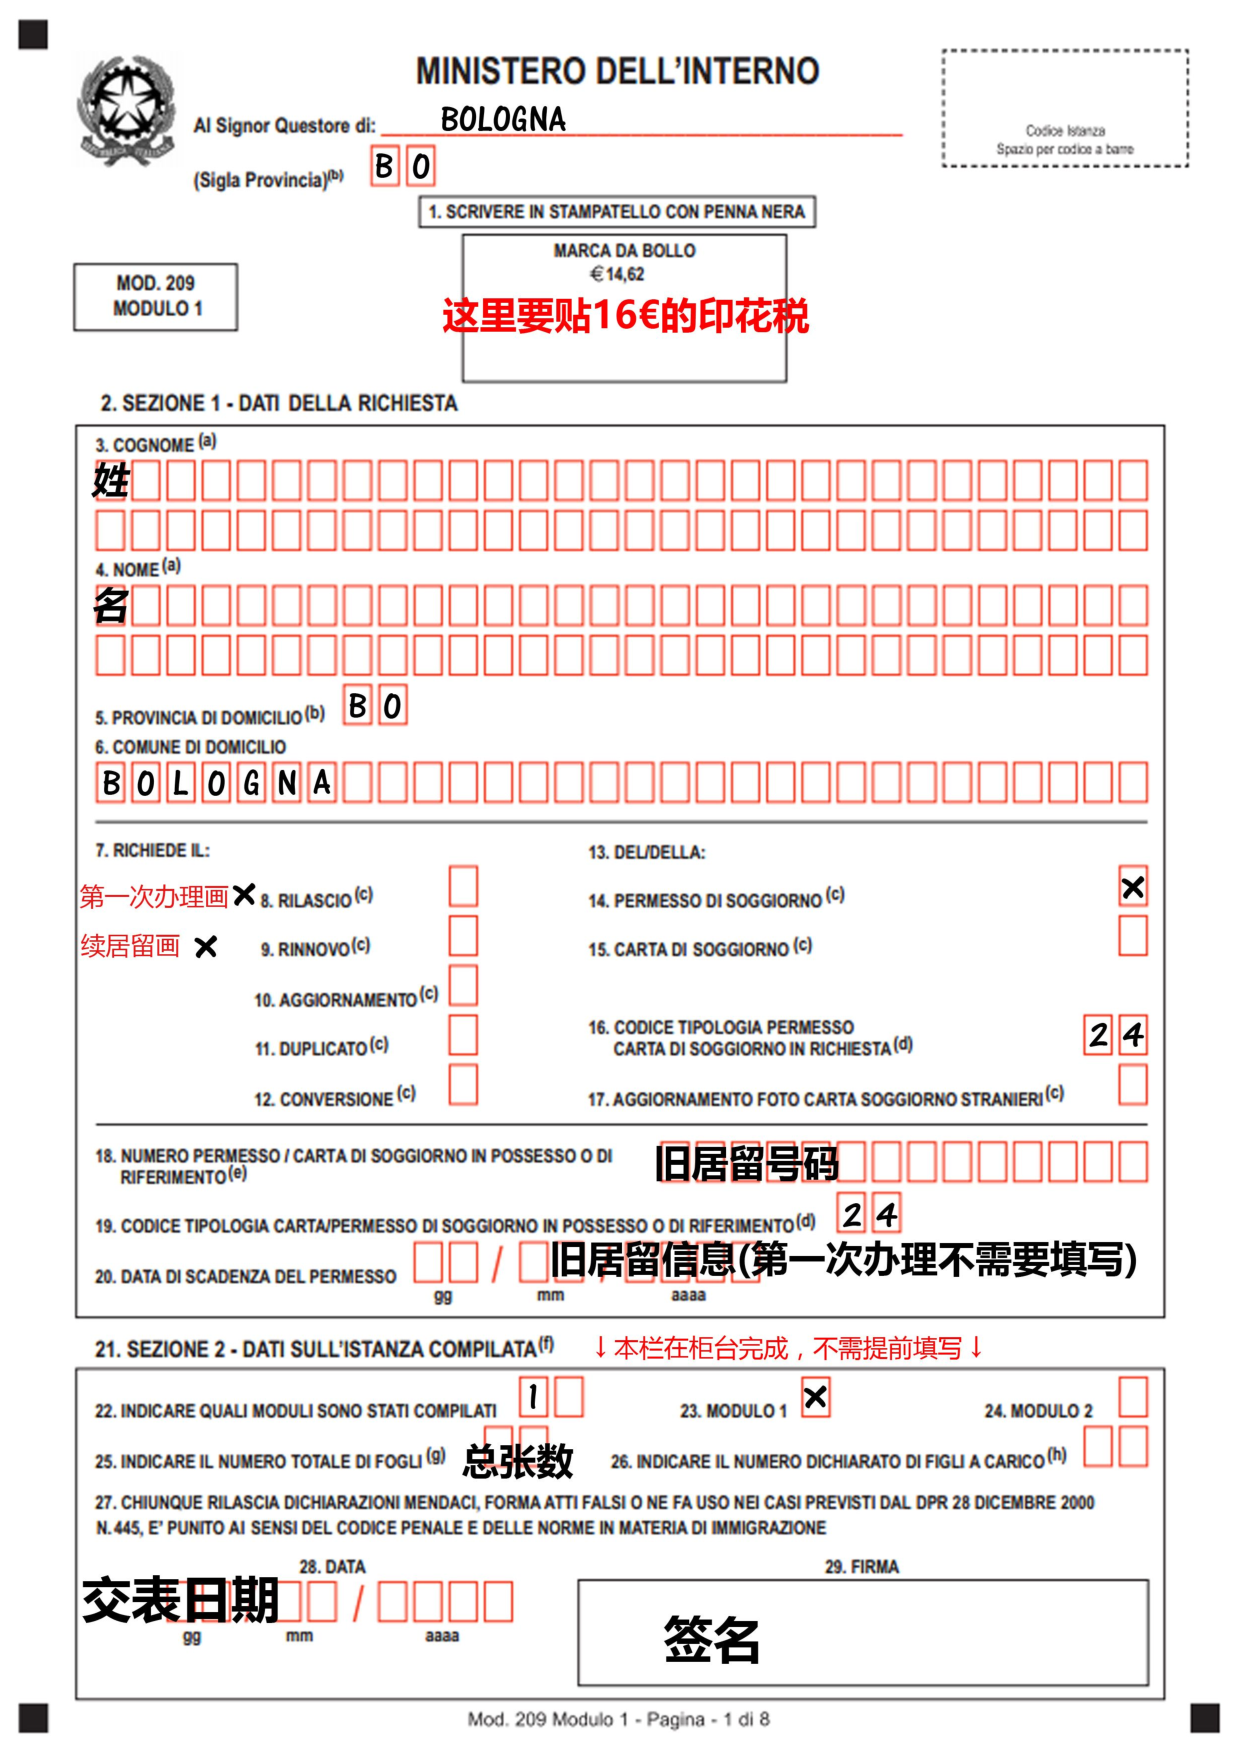
\includepdf{figures/jl1.pdf}
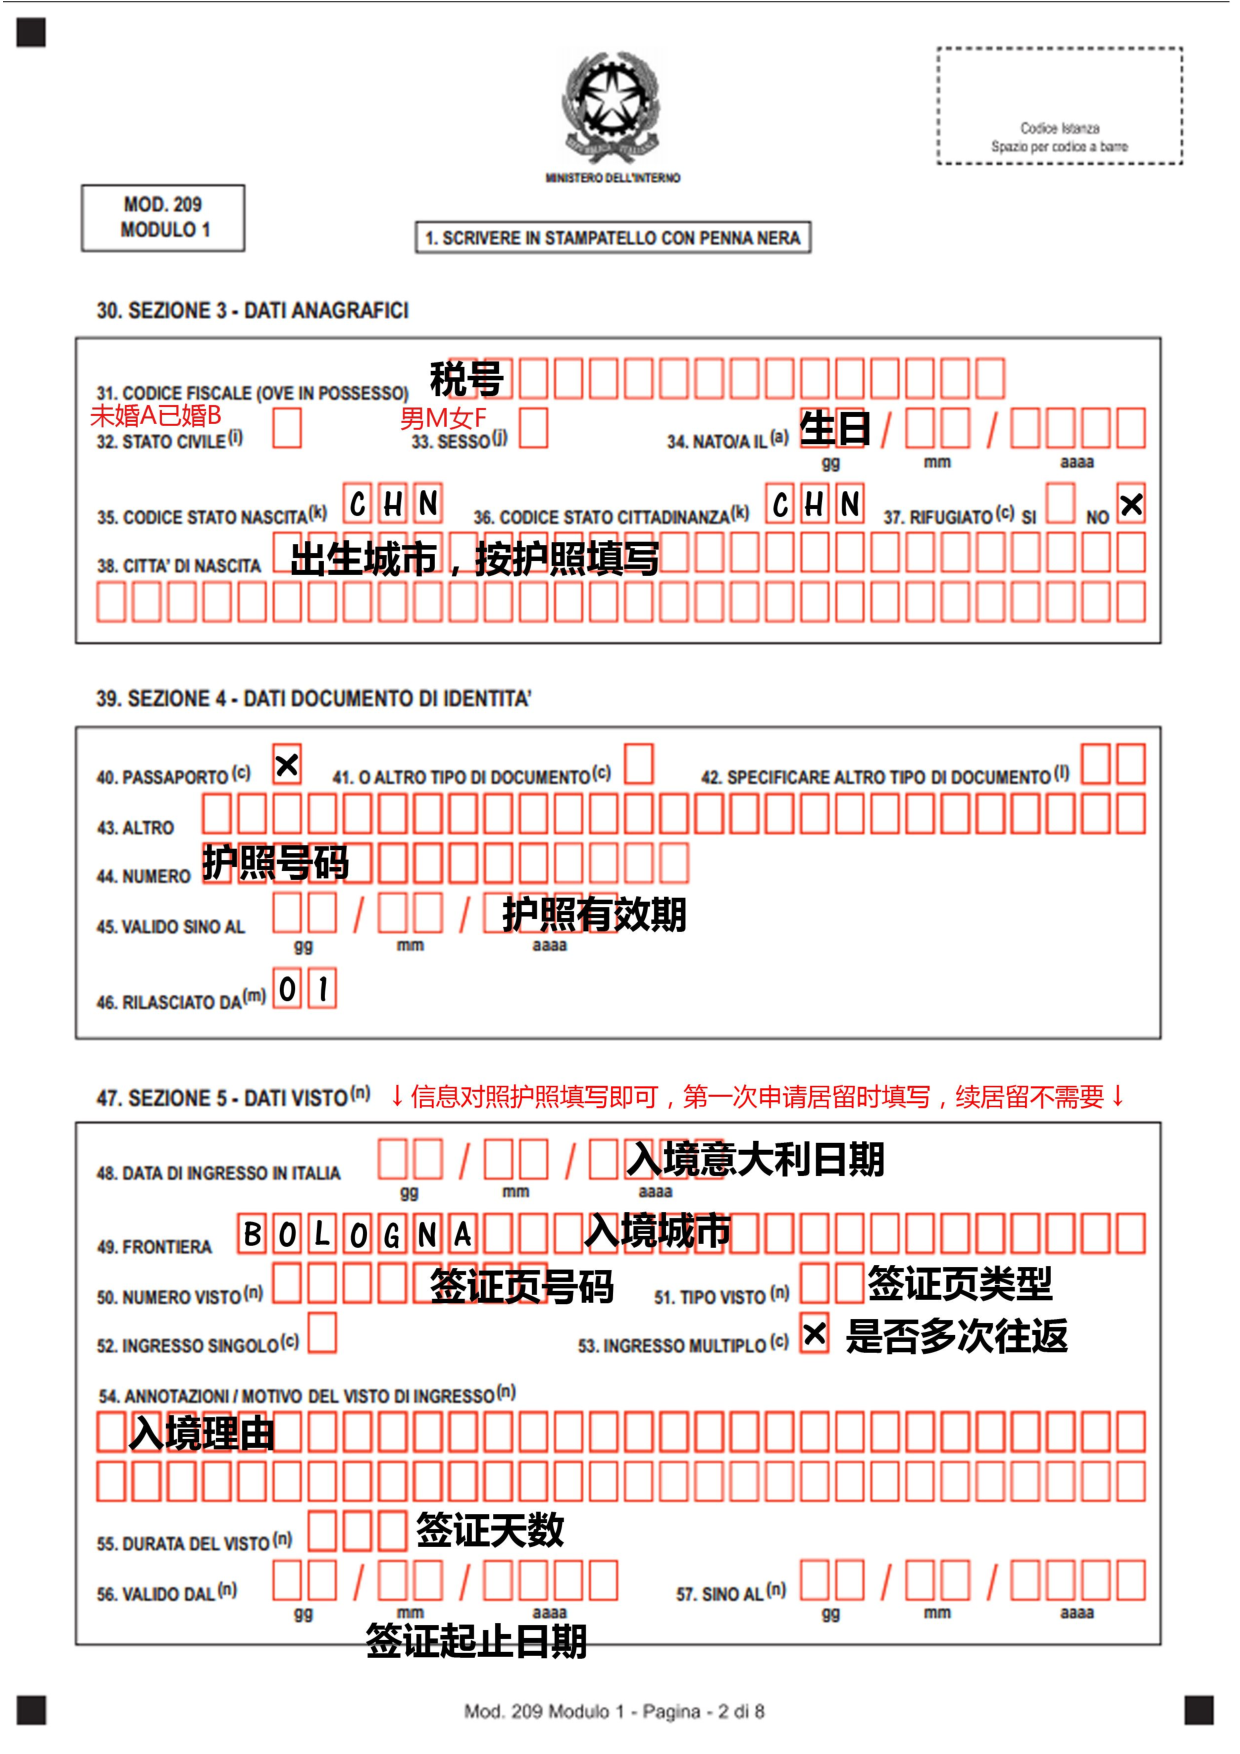
\includepdf{figures/jl2.pdf}
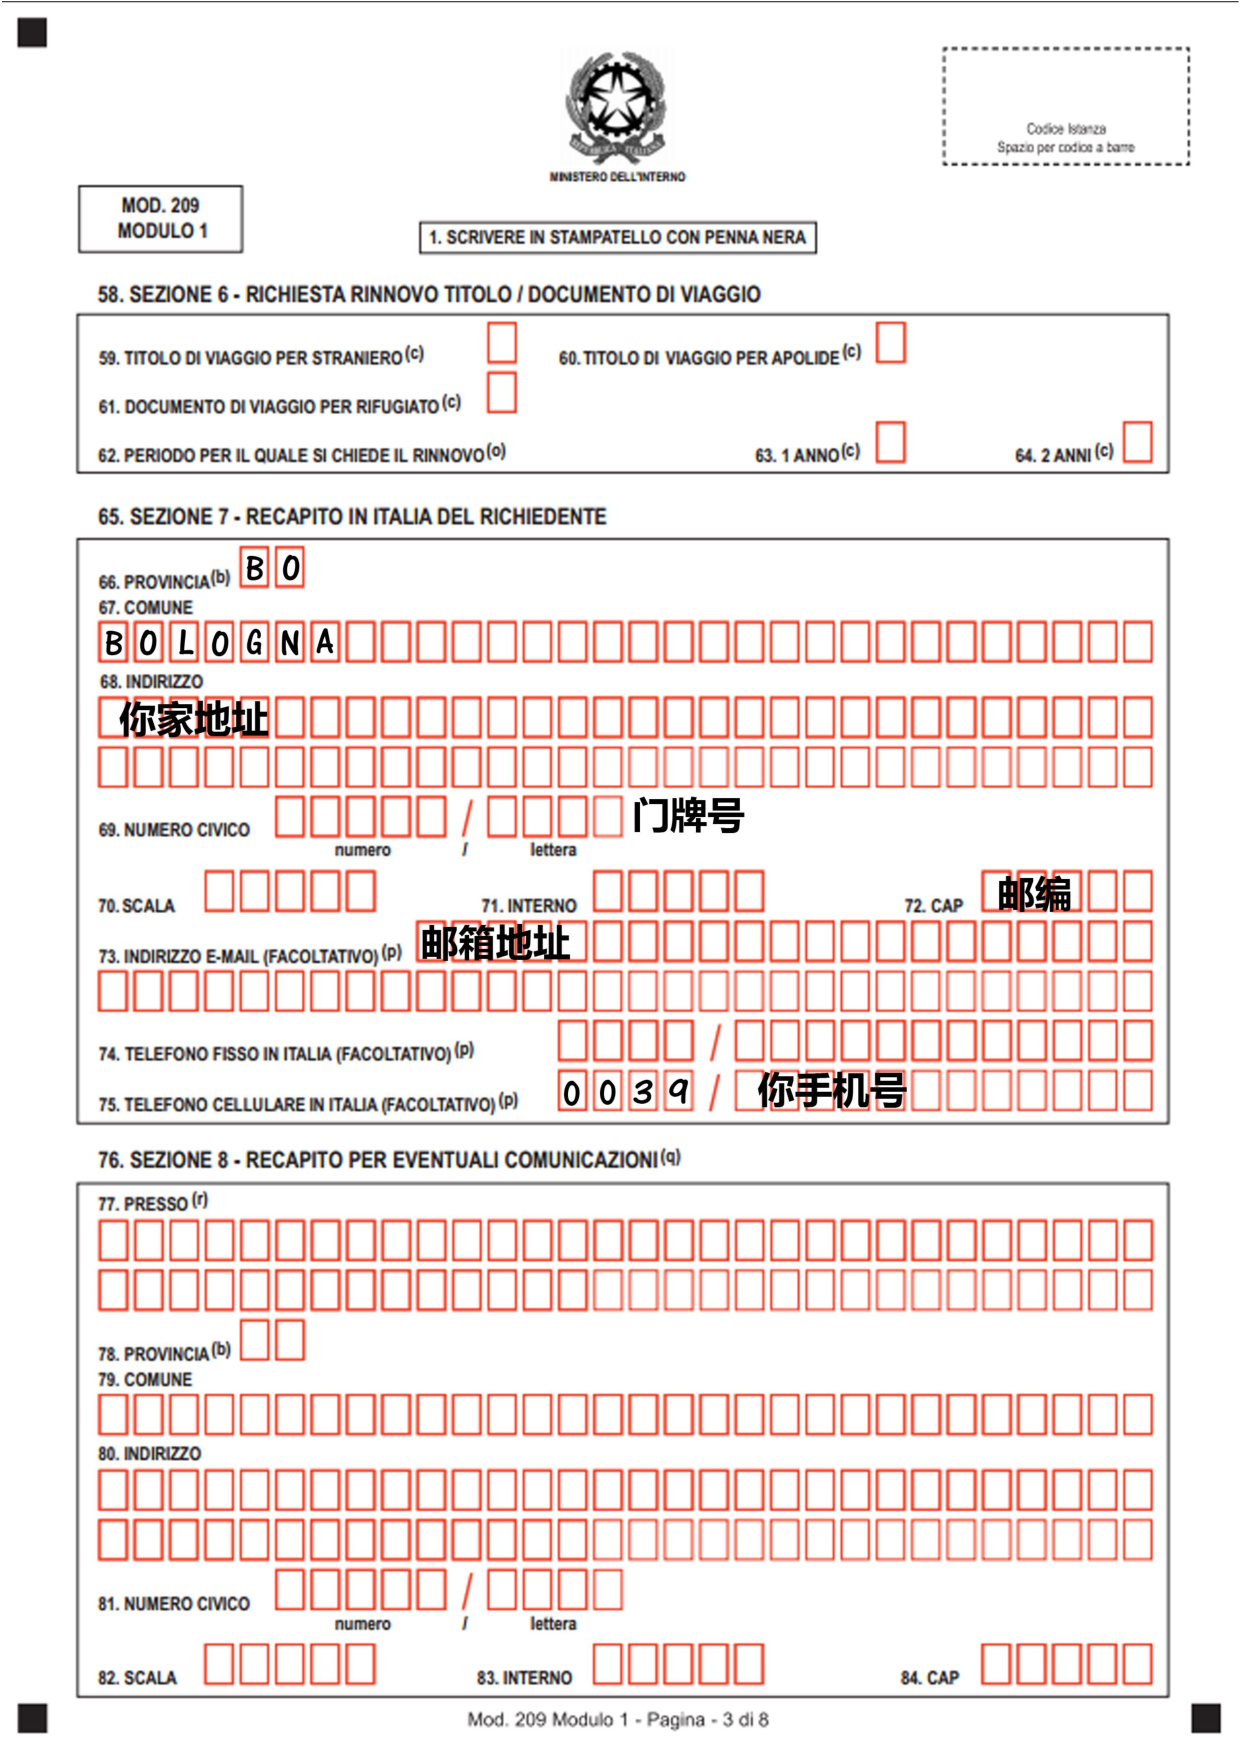
\includepdf{figures/jl3.pdf}
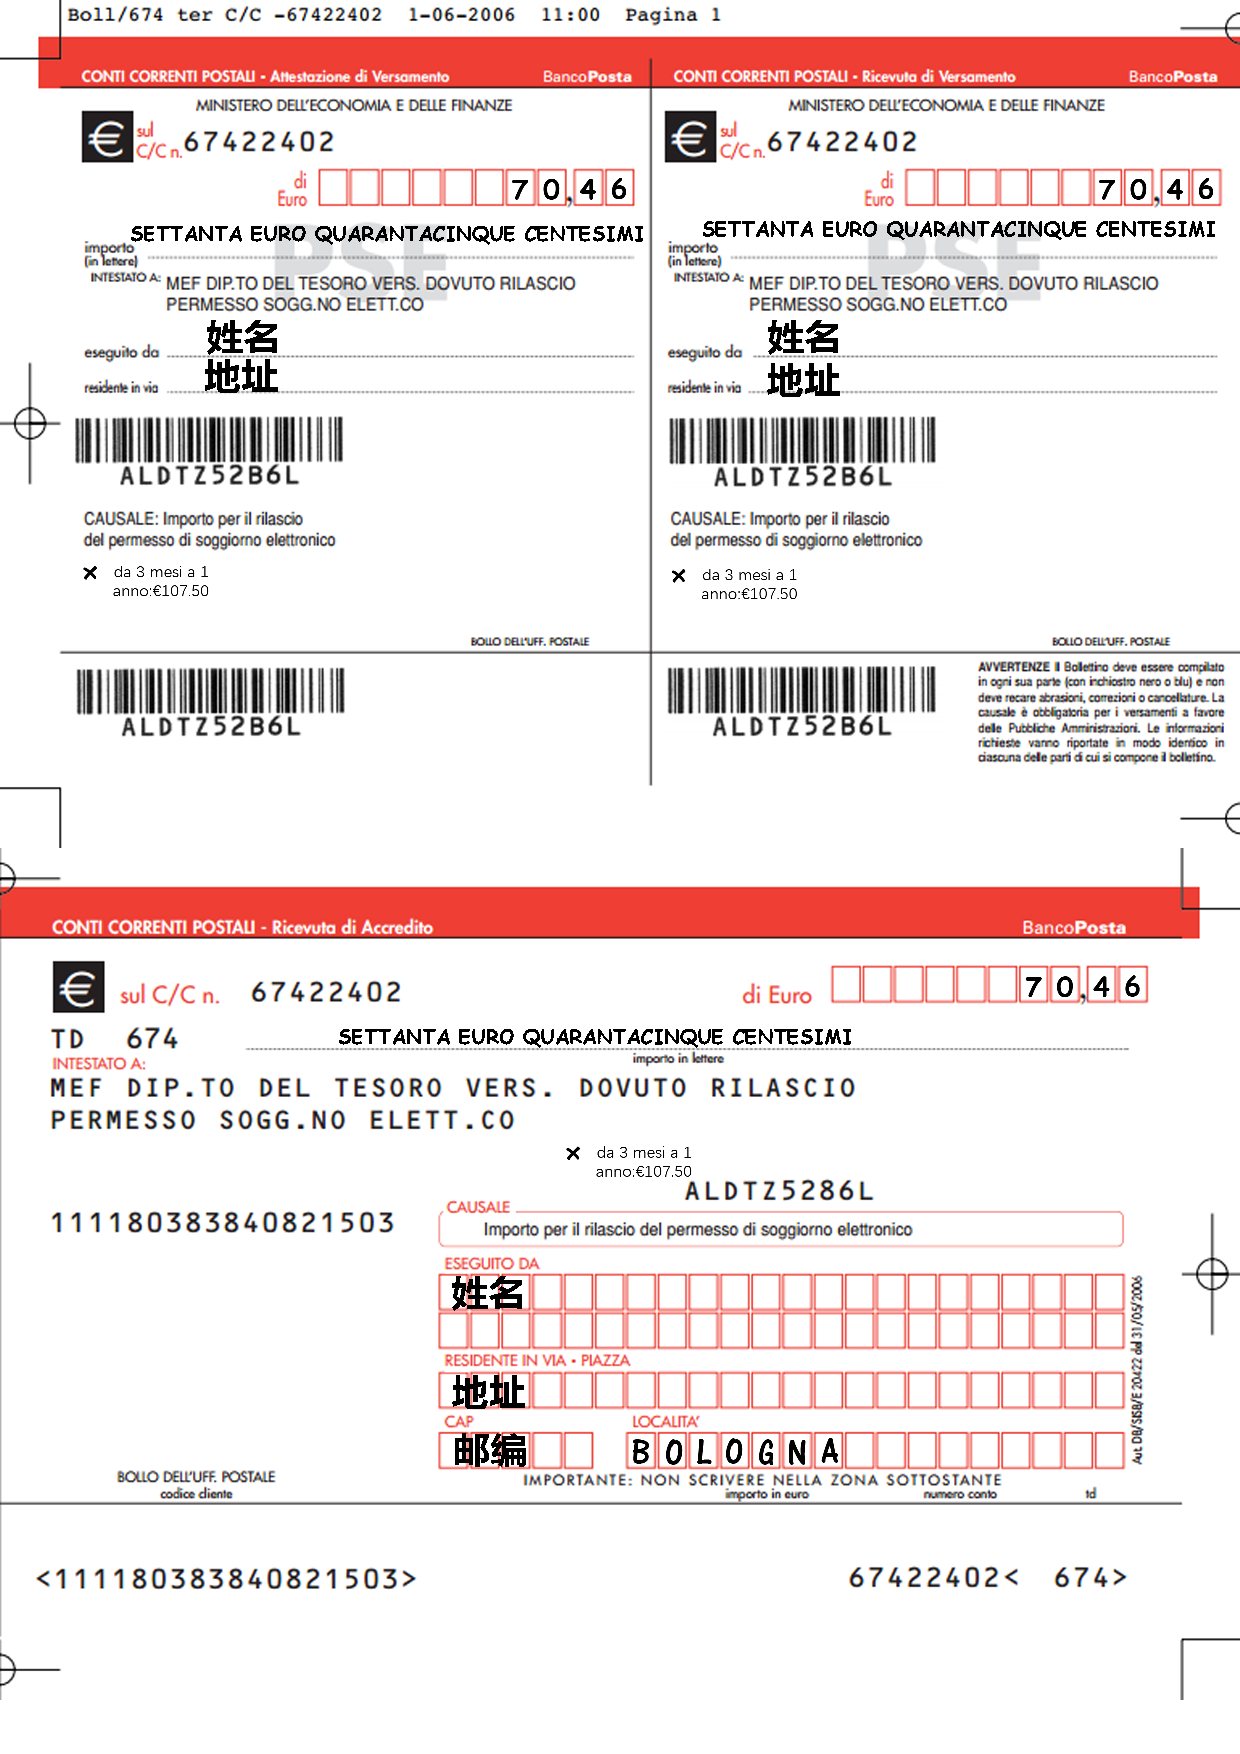
\includepdf{figures/jl4.pdf}
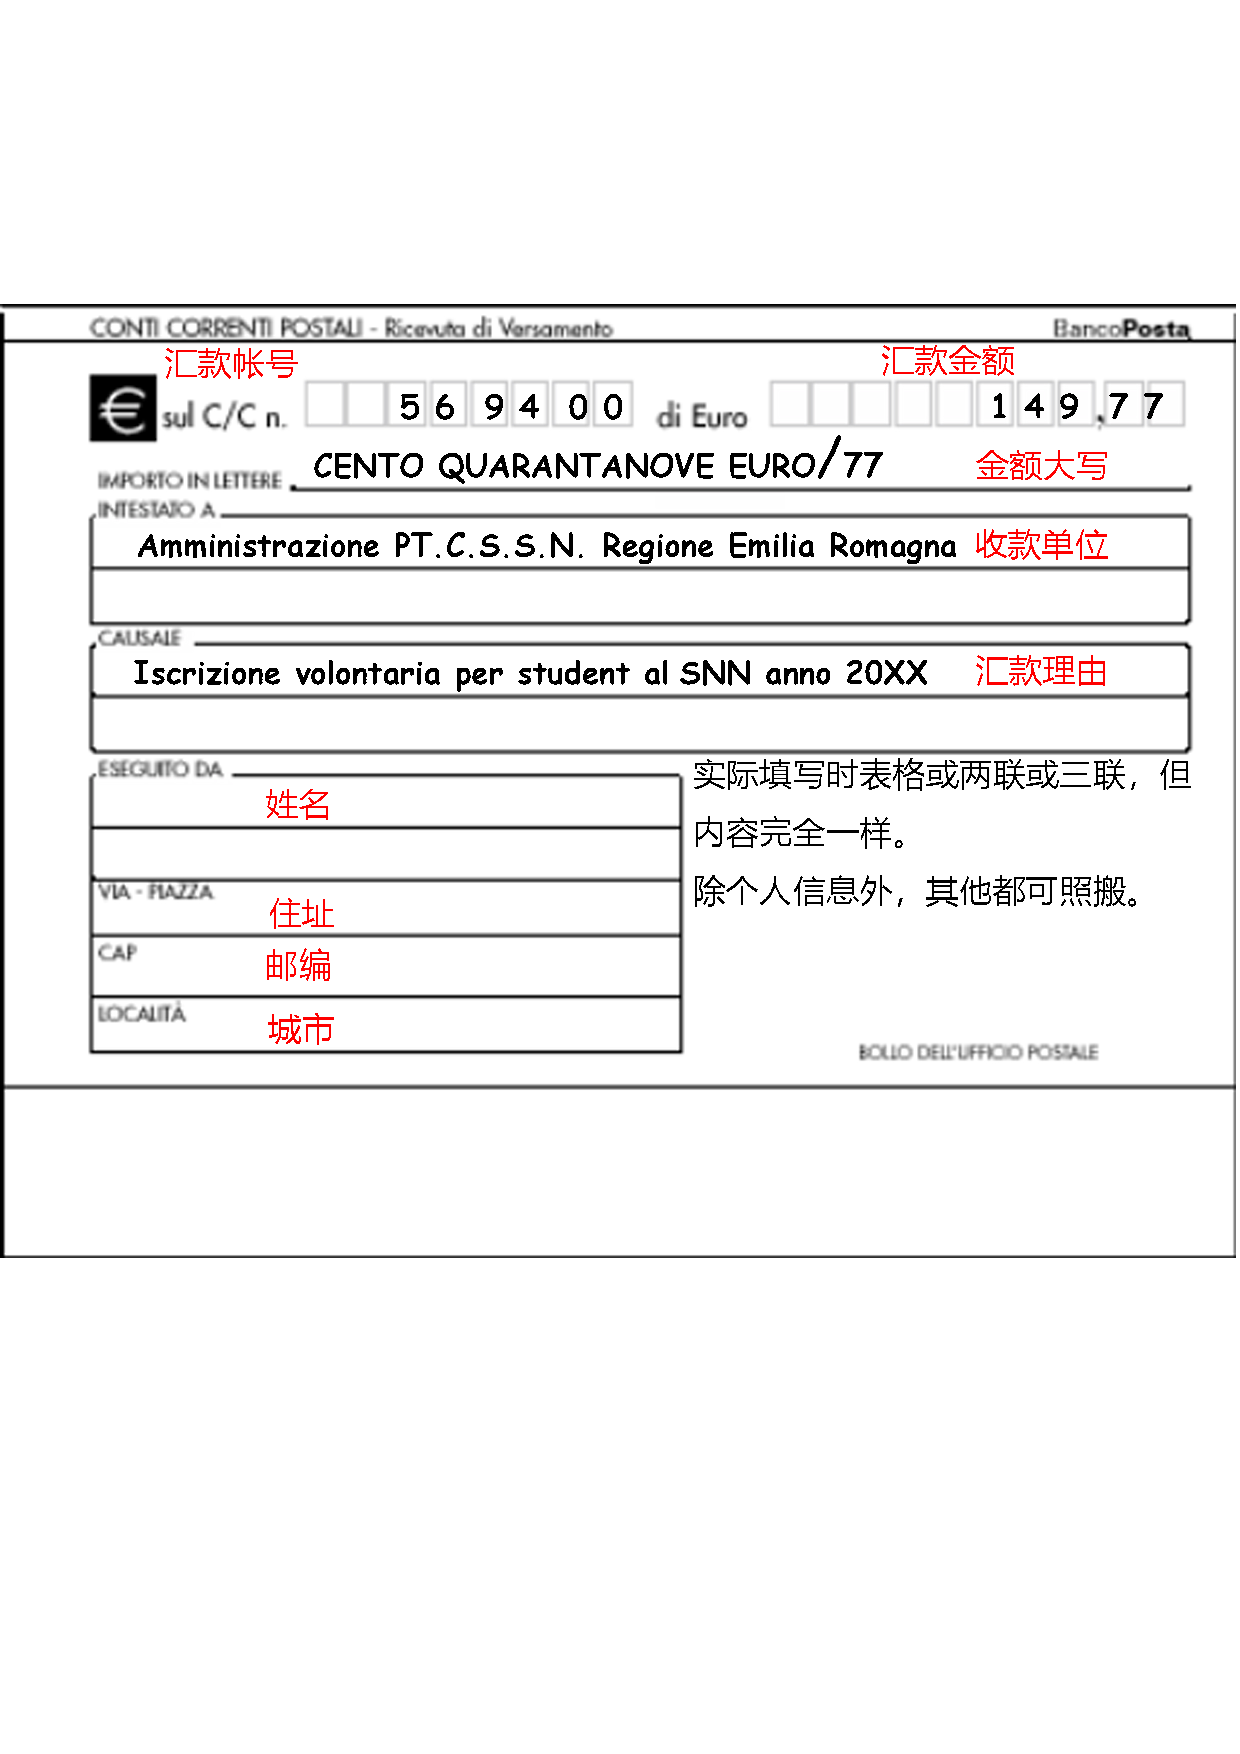
\includepdf{figures/jl5.pdf}

\rhead[\fancyplain{}{\bfseries \thechapter \:Appendix}]
{\fancyplain{}{\bfseries\thepage}}


%%%%%%%%%%%%%%%%%%%%%%%%%%%%%%%%%%%%%%%%%%%%%%%%%%%%%%%%%%%%%%%%%%%%%%%%%%%%%%%%%%
% 
%
%  ---     End First Appendix     ---
%
%
%%%%%%%%%%%%%%%%%%%%%%%%%%%%%%%%%%%%%%%%%%%%%%%%%%%%%%%%%%%%%%%%%%%%%%%%%%%%%%%%%%



%%%%%%%%%%%%%%%%%%%%%%%%%%%%%%%%%%%%%%%%%%%%%%%%%%%%%%%%%%%%%%%%%%%%%%%%%%%%%%%%%%
% 
%
%  ---     Second Appendix     ---
%
%
%%%%%%%%%%%%%%%%%%%%%%%%%%%%%%%%%%%%%%%%%%%%%%%%%%%%%%%%%%%%%%%%%%%%%%%%%%%%%%%%%%

\chapter{附录 B}     


\rhead[\fancyplain{}{\bfseries \thechapter \:Appendix}]
{\fancyplain{}{\bfseries\thepage}} 


%%%%%%%%%%%%%%%%%%%%%%%%%%%%%%%%%%%%%%%%%%%%%%%%%%%%%%%%%%%%%%%%%%%%%%%%%%%%%%%%%%
% 
%
%  ---     thebibliography     ---
%
%
%%%%%%%%%%%%%%%%%%%%%%%%%%%%%%%%%%%%%%%%%%%%%%%%%%%%%%%%%%%%%%%%%%%%%%%%%%%%%%%%%%


% \begin{thebibliography}{90}             %crea l'ambiente bibliografia
\rhead[\fancyplain{}{\bfseries \leftmark}]{\fancyplain{}{\bfseries
\thepage}}
%%%%%%%%%%%%%%%%%%%%%%%%%%%%%%%%%%%%%%%%%aggiunge la voce Bibliografia
                                        %   nell'indice
\addcontentsline{toc}{chapter}{参考链接}
\bibitem{irnerio}Irnerio Law https://en.wikipedia.org/wiki/Irnerius
\bibitem{cid}意大利身份证 http://www.comune.bologna.it/cittadino/servizi/9:2931/7422/
\bibitem{qs}QS世界大学排名 http://www.topuniversities.com/university-rankings
\bibitem{times}TIMES世界大学排名 https://www.timeshighereducation.com/world-university-rankings/2016/world-ranking
\bibitem{shanghai}上海交大世界大学排名 http://www.shanghairanking.cn/ARWU2015.html
\end{thebibliography}
 


%%%%%%%%%%%%%%%%%%%%%%%%%%%%%%%%%%%%%%%%%%%%%%%%%%%%%%%%%%%%%%%%%%%%%%%%%%%%%%%%%%
% 
%
%  ---     Ringraziamenti     ---
%
%
%%%%%%%%%%%%%%%%%%%%%%%%%%%%%%%%%%%%%%%%%%%%%%%%%%%%%%%%%%%%%%%%%%%%%%%%%%%%%%%%%%

% 
%%%%%%%%%%%%%%%%%%%%%%%%%%%%%%%%%%%%%%%%%%%%%%%%%%%%%%%%%%%%%%%%%%%%%%%%%%%%%%%%%%
% 
%
%  ---     Conclusions     ---
%
%
%%%%%%%%%%%%%%%%%%%%%%%%%%%%%%%%%%%%%%%%%%%%%%%%%%%%%%%%%%%%%%%%%%%%%%%%%%%%%%%%%%



% %%%%%%%%%%%%%%%%%%%%%%%%%%%%%%%%%%%%%%%%%non numera l'ultima pagina sinistra
% \clearpage{\pagestyle{empty}\cleardoublepage}
% %%%%%%%%%%%%%%%%%%%%%%%%%%%%%%%%%%%%%%%%%per fare le conclusioni
% \chapter*{鸣谢}


% %%%%%%%%%%%%%%%%%%%%%%%%%%%%%%%%%%%%%%%%%imposta l'intestazione di pagina
% \rhead[\fancyplain{}{\bfseries
% CONCLUSIONS}]{\fancyplain{}{\bfseries\thepage}}
% \lhead[\fancyplain{}{\bfseries\thepage}]{\fancyplain{}{\bfseries
% CONCLUSIONS}}
% %%%%%%%%%%%%%%%%%%%%%%%%%%%%%%%%%%%%%%%%%aggiunge la voce Conclusioni
%                                         %   nell'indice
% \addcontentsline{toc}{chapter}{结束语} 

% 手册制作不容易


\clearpage{\pagestyle{empty}\cleardoublepage}
\chapter*{感言}
\thispagestyle{empty}

手册制作不容易,需要一批热心的人,一批负责的人。前人种树,后人乘凉,我们就是要将这种团结无私的正能量发扬光大。
本手册完全开源,大家可以在 https://github.com/lteu/bo 地址下载到本版本源代码。\\\\
\noindent 本版手册由latex软件排版,由于技术,美工能力有限,手册未能达到彩色生动的效果。我们希望有善心,又精通indesign,photoshop的同学能贡献出自己的力量,让下版手册的颜值超越本版,同时证明自己的设计才能。 
% 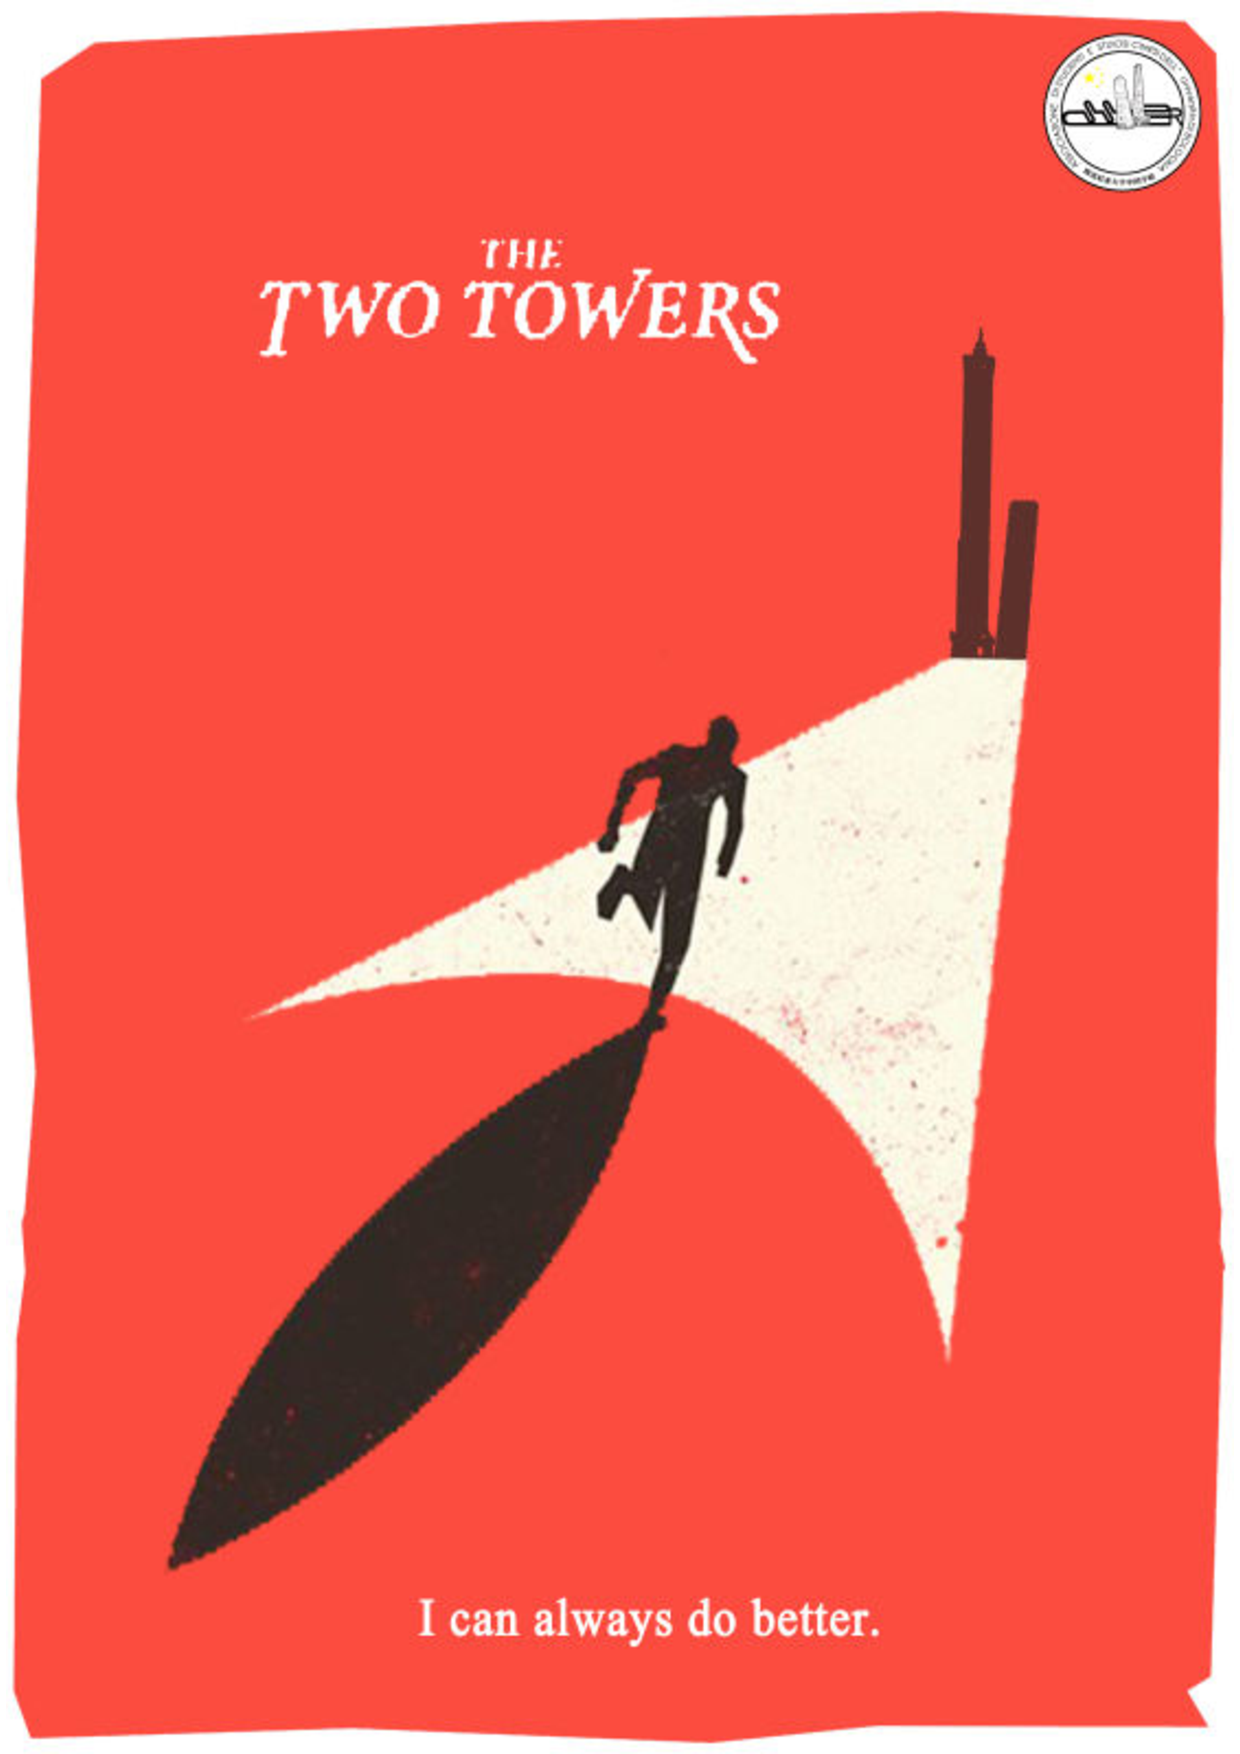
\includepdf{figures/cover2.pdf}
%%%%%%%%%%%%%%%%%%%%%%%%%%%%%%%%%%%%%%%%%%%%%%%%%%%%%%%%%%%%%%%%%%%%%%%%%%%%%%%%%%
% 
%
%  ---     End     ---
%
%
%%%%%%%%%%%%%%%%%%%%%%%%%%%%%%%%%%%%%%%%%%%%%%%%%%%%%%%%%%%%%%%%%%%%%%%%%%%%%%%%%%
\end{document}